\section{Noise Ceilings and Normalization}
\label{app:normalization}

Raw correlations and log-likelihood improvements are not comparable across datasets: a Pearson $r$ of 0.3 might be close to the achievable maximum in a noisy single-trial intracranial recording and far from it in a clean, heavily averaged fMRI dataset. The direct-prediction analyses therefore divide every dataset-unit score by a reference derived from the reliability of the human data, both in the Pareto composites and in Equation~\ref{eq:group}. They do not standardize outcomes by the spread of scores across models. Predictive composites take the median across dataset units within each response domain; regressions retain individual model--unit rows. Thus frontier membership and regression coefficients summarize different aspects of the data. We estimate two kinds of reference, one for each predictor track.

\subsection{Correlation ceilings: between-subject split-half reliability}
\label{app:corr-ceiling}

For every dataset where a model's score is a correlation between predicted and observed responses (at the level of an electrode, voxel, ROI, or channel), we estimate a noise ceiling from the split-half reliability of the human data, following \citet{vanbree2025noiseceiling}.

Our datasets typically present each item once to each participant, so there is no within-subject repetition to split on. We instead split \emph{across} subjects: for a given dataset and response unit, we repeatedly draw two random, equally sized halves of the subject pool, average each half's response per item, and correlate the two half-averages across items to obtain a split-half correlation $r_{\mathrm{half}}$, the group-average variant of split-half reliability that \citeauthor{vanbree2025noiseceiling} describe for designs without stimulus repetitions. We apply the Spearman--Brown correction to extrapolate from a half-sample to the full sample,
\[
r_{\mathrm{SB}} = \frac{2\,r_{\mathrm{half}}}{1 + r_{\mathrm{half}}},
\]
and average $r_{\mathrm{SB}}$ over many random subject splits to stabilize the estimate.

It is tempting to treat $r_{\mathrm{SB}}$ itself as the ceiling for a model's correlation with the data, but this is the mistake \citeauthor{vanbree2025noiseceiling} warn against: $r_{\mathrm{SB}}$ is a correlation between two noisy measurements, so by the classical correction-for-attenuation logic it bounds explained variance ($R^2$), not the correlation coefficient itself. A model that perfectly recovers the true signal is not itself noisy, so its correlation with the (still noisy) data is attenuated only once rather than twice, giving
\[
r_{\max} = \sqrt{r_{\mathrm{SB}}}.
\]
We therefore divide every model correlation by $\sqrt{r_{\mathrm{SB}}}$. Using $r_{\mathrm{SB}}$ as the ceiling for a raw correlation would systematically understate how far a model is from ceiling, especially at the low-to-intermediate reliability that characterizes most of our neural datasets. Ceilings are computed separately per response unit, using the same correlation family (Pearson or Spearman) as the corresponding model score, and response averaging and regional aggregation follow each dataset's scoring procedure. For Le Petit Prince the reference is a precomputed intersubject-correlation conversion. A correlation ratio is not explained variance, and differences between ratios should not be interpreted as percentage changes in predictive accuracy.

\subsection{Delta log-likelihood ceilings: the split-half design}
\label{app:dll-ceiling}

For the surprisal track, where the quantity of interest is the log-likelihood improvement $\Delta\ell$ that surprisal contributes over a nuisance-only baseline, a correlation-based ceiling does not directly apply. We instead adapt the split-half procedure that \citet{timkey2026dissociation} use to contextualize their filler-sentence regression models: we ask how much $\Delta\ell$ a predictor could achieve given only the information available to a single word-level scalar like surprisal, i.e.\ one value per item, with no participant- or trial-level access.

We construct this predictor directly from the data. For a given dataset, we randomly split the subject pool into two equal halves, $A$ and $B$. Within $A$, we compute the per-item mean response (averaged across subjects and, where relevant, electrodes), substitute it for surprisal in a mixed-effects model otherwise identical to the real full model, and fit it to half $B$. Comparing this model's held-out log likelihood with that of the baseline model (identical formula, predictor omitted) on the same $B$ data gives one estimate of the achievable $\Delta\ell$. We swap the halves, using $B$'s per-item means to predict $A$, sum the $\Delta\ell$ from both directions, and repeat over random splits (typically 15), reporting the mean per-observation $\Delta\ell$ as the reference. Two details carry over from the main fitting procedure: references are computed out of sample, using the same item or chunk train--test split as the corresponding real analysis, and the reference model's random-effects structure mirrors the real model's for that dataset, so the only difference between the two is the substitution of an empirical per-item mean for the model-derived surprisal. For datasets fit per region (Podcast, Pereira), the reference is computed per region and each region's score is normalized by its own reference before the regions are combined.

Because the substitute predictor is a finite-sample group average rather than a noise-free oracle, it is not an upper bound in the strict sense. The reference can be small, uncertain, or exceeded by a model scored against a fuller response average, particularly when there are few subjects per item or the achievable $\Delta\ell$ is very small. Ratios above one are therefore retained and do not establish superhuman prediction. The same issue applies to the split-half references used in RDM regression (Appendix~\ref{app:rsa}). Neither these ratios nor their cross-dataset medians are fractions of explainable variance.

\subsection{Reported ceilings and score ranges}
\label{app:ceiling-values}

Tables~\ref{tab:corr-ceilings} and~\ref{tab:dll-ceilings} report every reference used in the final-layer direct-prediction scores, with the largest normalized score among the 118 models and the number of models above the reference. For the embedding track, no model exceeds its ceiling; the best models reach between about 12\% and 78\% of the ceiling, and are furthest from it for Natural Stories fMRI and the continuous neural recordings (MEG-MASC, Podcast, Broderick). For the surprisal track, four references (UCL self-paced reading, Broderick, Federmeier et al.\ 2007, Hubbard et al.\ 2019; marked $\dagger$) are exceeded by many models or have a split-to-split SD larger than half their value; they rest on few subjects per item or on a very small achievable $\Delta\ell$, and normalized scores on them should be interpreted with that in mind. A low reference indicates that the human measurement itself carries limited reliable signal at the item level.

Table~\ref{tab:score-ranges} reports the resulting normalized scores. Neural surprisal scores have markedly different ranges across datasets: Federmeier 2007 spans approximately $-3.44$ to $6.98$, whereas MEG-MASC spans approximately $-.013$ to $.007$. These differences motivate caution about pooled domain coefficients: a dataset random intercept absorbs location differences, not differences in residual scale or uncertain denominators. Appendix~\ref{app:robustness} therefore refits the group analysis without the flagged units, with winsorized scores, on a within-unit robust z-score, and leaving out one unit at a time.

{\setlength{\tabcolsep}{5pt}
\begin{longtable}{@{}lccc@{}}
\caption{Split-half correlation noise ceilings (BrainScore normalization, $\sqrt{r_{\mathrm{SB}}}$, Appendix~\ref{app:corr-ceiling}) for every dataset in the embedding/ridge track, and the fraction of that ceiling reached by the best model. Rows marked $\dagger$ have a ceiling below 0.01 -- an absolute reliability so low that a high percent-of-ceiling figure reflects very little recoverable signal in the human data itself, not a strong model fit; we report these for completeness but do not treat them as headline results.}
\label{tab:corr-ceilings} \\
\toprule
\textbf{Dataset} & \textbf{Modality} & \textbf{Ceiling ($\sqrt{r_{\mathrm{SB}}}$)} & \textbf{Best model's \% of ceiling} \\
\midrule
\endfirsthead
\multicolumn{4}{c}{\tablename\ \thetable{} -- continued} \\
\toprule
\textbf{Dataset} & \textbf{Modality} & \textbf{Ceiling ($\sqrt{r_{\mathrm{SB}}}$)} & \textbf{Best model's \% of ceiling} \\
\midrule
\endhead
\midrule \multicolumn{4}{r}{\textit{continued on next page}} \\
\endfoot
\bottomrule
\endlastfoot
ZuCo Reading SR & Behavioral & 0.819 & 81\% \\
ZuCo Reading & Behavioral & 0.819 & 79\% \\
MECO SP & Behavioral & 0.930 & 79\% \\
MECO & Behavioral & 0.899 & 72\% \\
Provo SP & Behavioral & 0.943 & 69\% \\
Provo & Behavioral & 0.933 & 68\% \\
GECO & Behavioral & 0.627 & 65\% \\
ZuCo Reading TSR & Behavioral & 0.819 & 65\% \\
GECO GP & Behavioral & 0.529 & 62\% \\
OneStop SP & Behavioral & 0.888 & 62\% \\
UCL Reading & Behavioral & 0.689 & 56\% \\
Natural Stories SPR & Behavioral & 0.914 & 55\% \\
MECO GP & Behavioral & 0.684 & 51\% \\
OneStop & Behavioral & 0.829 & 51\% \\
Le Petit Prince fMRI & fMRI & 0.912 & 49\% \\
Provo GP & Behavioral & 0.919 & 47\% \\
Fedorenko2016 ECoG & ECoG & 0.711 & 40\% \\
OneStop GP & Behavioral & 0.776 & 38\% \\
Nieuwland N400 EEG & EEG (N400) & 0.344 & 35\% \\
Tuckute fMRI & fMRI & 0.480 & 34\% \\
Pereira fMRI & fMRI & 0.507 & 30\% \\
Natural Stories fMRI & fMRI & 0.628 & 28\% \\
Podcast iEEG & iEEG & 0.398 & 23\% \\
Broderick EEG & EEG & 0.108 & 22\% \\
MEG-MASC (Gwilliams) & MEG & 0.097 & 20\% \\
MEG-MASC (Gwilliams) & MEG & 0.097 & 20\% \\
\end{longtable}
}


{\small\setlength{\tabcolsep}{4pt}
\begin{longtable}{@{}lrrrrr@{}}
\caption{Split-half likelihood references used in final-layer surprisal normalization, in $\Delta\ell$ per observation. SD is variability across splits or iterations, not a standard error; -- means the aggregate file supplies no such value. Splits reports successful/attempted draws where available. Above is the number of finite model scores exceeding the reference, and Maximum is the largest normalized score. A dagger flags split SD/reference $>.5$ or more than 10\% of models above one; this is a descriptive diagnostic, not an exclusion rule. Pereira split counts apply to each of its two ROIs; region-specific references are detailed in the text.}\label{tab:dll-ceilings} \\
\toprule
Dataset / measure & Reference & SD & Splits & Above & Maximum \\
\midrule
\endfirsthead
\multicolumn{6}{c}{\tablename\ \thetable{} -- continued} \\
\toprule
Dataset / measure & Reference & SD & Splits & Above & Maximum \\
\midrule
\endhead
\midrule\multicolumn{6}{r}{Continued on next page} \\
\endfoot
\bottomrule
\endlastfoot
GECO FP & $8.66\times10^{-3}$ & $3.59\times10^{-4}$ & 10/10 & 0/118 & 0.272 \\
GECO GP & $4.16\times10^{-3}$ & $4.30\times10^{-4}$ & 15/15 & 0/118 & 0.183 \\
MECO FP & $2.34\times10^{-2}$ & $3.68\times10^{-3}$ & 15/15 & 0/118 & 0.172 \\
MECO GP & $7.97\times10^{-3}$ & $1.86\times10^{-3}$ & 15/15 & 0/118 & 0.089 \\
MECO SP & $3.79\times10^{-2}$ & $2.56\times10^{-3}$ & 15/15 & 0/118 & 0.190 \\
Natural Stories SPR & $2.38\times10^{-2}$ & $9.14\times10^{-4}$ & 15/15 & 0/118 & 0.395 \\
OneStop FP & $1.29\times10^{-2}$ & $5.59\times10^{-4}$ & 15/15 & 0/118 & 0.379 \\
OneStop GP & $1.43\times10^{-2}$ & $8.90\times10^{-4}$ & 15/15 & 0/118 & 0.091 \\
OneStop SP & $2.36\times10^{-2}$ & $1.39\times10^{-3}$ & 15/15 & 0/118 & 0.373 \\
Provo FP & $3.35\times10^{-2}$ & $1.50\times10^{-3}$ & 15/15 & 0/118 & 0.138 \\
Provo GP & $3.60\times10^{-2}$ & $1.60\times10^{-3}$ & 15/15 & 0/118 & 0.064 \\
Provo SP & $4.57\times10^{-2}$ & $1.02\times10^{-3}$ & 15/15 & 0/118 & 0.194 \\
UCL SPR$\dagger$ & $2.36\times10^{-3}$ & $2.61\times10^{-4}$ & 15/15 & 51/118 & 1.503 \\
ZuCo NR & $2.78\times10^{-2}$ & $2.25\times10^{-3}$ & 10/10 & 0/118 & 0.311 \\
ZuCo SR & $3.14\times10^{-2}$ & $1.55\times10^{-3}$ & 15/15 & 0/118 & 0.454 \\
ZuCo TSR & $1.25\times10^{-2}$ & $2.39\times10^{-3}$ & 15/15 & 0/118 & 0.629 \\
Le Petit Prince fMRI & $1.01\times10^{-2}$ & $8.79\times10^{-4}$ & 15/15 & 0/118 & 0.057 \\
Natural Stories fMRI & $2.97\times10^{-2}$ & $3.94\times10^{-3}$ & 15/15 & 0/118 & 0.134 \\
Pereira fMRI & $2.37\times10^{-2}$ & -- & 29/30 & 0/118 & 0.640 \\
Tuckute fMRI & $9.52\times10^{-3}$ & $1.32\times10^{-3}$ & 10/10 & 0/118 & 0.248 \\
Fedorenko intracranial & $8.32\times10^{-3}$ & $1.62\times10^{-3}$ & 10/10 & 4/118 & 1.150 \\
Podcast ECoG & $6.19\times10^{-3}$ & -- & -- & 0/118 & 0.118 \\
Broderick EEG$\dagger$ & $1.00\times10^{-4}$ & $7.00\times10^{-5}$ & 60/60 & 42/118 & 2.293 \\
MEG-MASC & $7.31\times10^{-4}$ & $1.78\times10^{-4}$ & 15/15 & 0/118 & 0.007 \\
Nieuwland N400 & $1.25\times10^{-2}$ & $1.20\times10^{-3}$ & 30/30 & 0/118 & 0.342 \\
Federmeier 2007 N400$\dagger$ & $2.61\times10^{-3}$ & $2.75\times10^{-3}$ & 15/15 & 67/118 & 6.976 \\
Hubbard 2019 N400$\dagger$ & $2.22\times10^{-3}$ & $1.21\times10^{-3}$ & 15/15 & 49/118 & 2.607 \\
\end{longtable}
}


\begin{table}[p]
\centering\small
\caption{Normalized final-layer scores of the direct-prediction analyses. Each entry is minimum / median / maximum across available models in that unit. These ranges describe the input tables before any further complete-case filtering for the regression.}
\label{tab:score-ranges}
\begin{tabular}{lrr}
\toprule
Dataset unit & Embeddings & Surprisal\\
\midrule
Broderick EEG & 0.005 / 0.111 / 0.148 & -0.077 / 0.341 / 2.293 \\
Fedorenko intracranial & 0.078 / 0.247 / 0.291 & -0.239 / 0.155 / 1.150 \\
GECO FP & 0.408 / 0.543 / 0.587 & 0.021 / 0.205 / 0.272 \\
GECO GP & 0.370 / 0.483 / 0.543 & 0.002 / 0.108 / 0.183 \\
Le Petit Prince fMRI & 0.038 / 0.383 / 0.447 & -0.026 / 0.010 / 0.057 \\
MECO FP & 0.471 / 0.587 / 0.650 & -0.004 / 0.069 / 0.172 \\
MECO GP & 0.266 / 0.377 / 0.453 & -0.182 / 0.003 / 0.089 \\
MECO SP & 0.535 / 0.648 / 0.737 & 0.005 / 0.070 / 0.190 \\
MEG-MASC & 0.026 / 0.097 / 0.129 & -0.013 / -0.004 / 0.007 \\
Natural Stories SPR & 0.193 / 0.344 / 0.450 & 0.151 / 0.263 / 0.395 \\
Nieuwland N400 & -0.362 / 0.214 / 0.425 & -0.608 / 0.028 / 0.342 \\
Natural Stories fMRI & 0.015 / 0.068 / 0.120 & 0.024 / 0.064 / 0.134 \\
OneStop FP & 0.282 / 0.383 / 0.422 & 0.007 / 0.214 / 0.379 \\
OneStop GP & 0.212 / 0.273 / 0.310 & 0.011 / 0.057 / 0.091 \\
OneStop SP & 0.339 / 0.464 / 0.523 & 0.017 / 0.231 / 0.373 \\
Pereira fMRI & 0.116 / 0.203 / 0.238 & -0.157 / 0.219 / 0.640 \\
Podcast ECoG & 0.030 / 0.125 / 0.157 & 0.013 / 0.088 / 0.118 \\
Provo FP & 0.394 / 0.517 / 0.604 & 0.012 / 0.068 / 0.138 \\
Provo GP & 0.234 / 0.341 / 0.403 & 0.001 / 0.033 / 0.064 \\
Provo SP & 0.407 / 0.527 / 0.608 & 0.007 / 0.131 / 0.194 \\
Federmeier 2007 N400 & 0.149 / 0.519 / 0.746 & -3.436 / 3.138 / 6.976 \\
Hubbard 2019 N400 & 0.044 / 0.515 / 0.777 & -1.099 / 0.743 / 2.607 \\
Tuckute fMRI & 0.025 / 0.223 / 0.299 & -0.031 / 0.121 / 0.248 \\
UCL SPR & 0.205 / 0.316 / 0.470 & 0.075 / 0.984 / 1.503 \\
ZuCo NR & 0.615 / 0.693 / 0.741 & -0.017 / 0.196 / 0.311 \\
ZuCo SR & 0.565 / 0.696 / 0.757 & 0.038 / 0.333 / 0.454 \\
ZuCo TSR & 0.479 / 0.555 / 0.598 & 0.157 / 0.319 / 0.629 \\
\bottomrule\end{tabular}\end{table}


\section{Full List of Evaluated Models}
\label{app:models}

Table~\ref{tab:models} lists every model evaluated in this benchmark, with its family, depth, parameter count, and HuggingFace repository, organized into the four groups of Section~\ref{sec:design-models}. The main comparison uses released model instances rather than intermediate training checkpoints. The four groups contain 59, 24, 11, and 24 models, respectively, for Standard LLMs, Memory-Constrained, BabyLM, and Constrained-BabyLM. The direct-prediction regressions retain 115 models after requiring usable scores and perplexity. Architectural depth metadata can include an embedding state in some implementations; the analysis consistently uses the final representation available in the corresponding evaluation.

The Memory-Constrained and Constrained-BabyLM groups (identical small architectures, web-scale vs.\ BabyLM-scale training data) cover several mechanisms: architectures that bias attention toward nearby tokens through a fixed distance penalty, ALiBi \citep{press2021train,devarda2024locally,clark2025linear}; architectures that replace softmax attention with a content-sensitive forget gate \citep{lin2025forgetting} or a stick-breaking process \citep{tan2025scaling}; and hard local $n$-gram windows that can only attend to the two, three, or five preceding tokens regardless of the input \citep{bu2026staticlinearattentionconstraints}. The web-scale group additionally contains CBR-RNN and its variant CBR-RNN-M, a small recurrent architecture with a bounded context representation \citep{timkey2023limited}, and larger web-scale models built on the same mechanisms (BLOOM with ALiBi, the Forgetting Transformer, and MoLM). The small architectures and their BabyLM-scale counterparts were obtained from the public HuggingFace checkpoints released alongside \citet{bu2026staticlinearattentionconstraints}. The BabyLM group spans submissions and baselines from the BabyLM shared tasks, including the organizers' baselines \citep{charpentier2025findings}, a masked-language-modeling variant \citep{edman2025mask}, an instruction-tuned small model \citep{capone2025classit}, a mixture-of-experts architecture \citep{tapaninaho2025moep}, and a model trained with interactive storytelling feedback \citep{martins2025upon}, alongside the earlier BabyLM challenges \citep{warstadt2023cfp,warstadt2023findings,hu2024secondbabylm}, all obtained from their public HuggingFace repositories. The Standard LLM group spans off-the-shelf families with no human-inspired constraint on either architecture or training data: GPT-2 \citep{radford2019gpt2}, GPT-Neo \citep{black2021gptneo}, OPT \citep{zhang2022opt}, Mamba and Mamba-2 \citep{gu2024mamba}, RWKV-4, Pythia \citep{biderman2023pythia}, OLMo-2 \citep{olmo20252olmo2furious}, Qwen3 \citep{qwen3}, Llama-3, Ministral, and the attention baselines of the Forgetting Transformer \citep{lin2025forgetting}, from 14 million to 66 billion parameters and including both Transformer and state-space architectures.

{\setlength{\tabcolsep}{3pt}
\begin{longtable}{@{}p{1.38cm}p{5.22cm}cccc@{}}
\caption{All models evaluated in this benchmark, grouped by family within the three model classes of Section~3.2 (rules separate each fine-grained family). Parameter and layer counts follow the originating release (or the loaded config for the memory-constrained and BabyLM checkpoints; see \texttt{neuroai/models/registry.py}). Training-token/word counts are reported only where documented with confidence by the originating source; a blank cell means this was not reliably available rather than zero. For Pythia and OLMo-2, the listed repository is evaluated both at its final (\texttt{main}) checkpoint and at multiple intermediate training steps (Section~3.2).}
\label{tab:models} \\
\toprule
\textbf{Family} & \textbf{HuggingFace model ID} & \textbf{\#Params} & \textbf{\#Layers} & \textbf{Tr. tokens} & \textbf{Ref.} \\
\midrule
\endfirsthead
\multicolumn{6}{c}{\tablename\ \thetable{} -- continued} \\
\toprule
\textbf{Family} & \textbf{HuggingFace model ID} & \textbf{\#Params} & \textbf{\#Layers} & \textbf{Tr. tokens} & \textbf{Ref.} \\
\midrule
\endhead
\midrule \multicolumn{6}{r}{\textit{continued on next page}} \\
\endfoot
\bottomrule
\endlastfoot
\multicolumn{6}{l}{\textbf{Standard LLMs}} \\
\midrule
\scriptsize GPT-2 & \textcolor{blue}{\ttfamily\fontsize{7.0}{8.4}\selectfont\seqsplit{openai-community/gpt2}} & \scriptsize 124M & \scriptsize 13 & \scriptsize  & \scriptsize \citep{radford2019gpt2} \\
\scriptsize GPT-2 & \textcolor{blue}{\ttfamily\fontsize{7.0}{8.4}\selectfont\seqsplit{openai-community/gpt2-medium}} & \scriptsize 355M & \scriptsize 25 & \scriptsize  & \scriptsize \citep{radford2019gpt2} \\
\scriptsize GPT-2 & \textcolor{blue}{\ttfamily\fontsize{7.0}{8.4}\selectfont\seqsplit{openai-community/gpt2-large}} & \scriptsize 774M & \scriptsize 37 & \scriptsize  & \scriptsize \citep{radford2019gpt2} \\
\scriptsize GPT-2 & \textcolor{blue}{\ttfamily\fontsize{7.0}{8.4}\selectfont\seqsplit{openai-community/gpt2-xl}} & \scriptsize 1.6B & \scriptsize 49 & \scriptsize  & \scriptsize \citep{radford2019gpt2} \\
\midrule
\scriptsize GPT-Neo/J/NeoX & \textcolor{blue}{\ttfamily\fontsize{7.0}{8.4}\selectfont\seqsplit{EleutherAI/gpt-neo-125m}} & \scriptsize 125M & \scriptsize 13 & \scriptsize  & \scriptsize \citep{black2021gptneo} \\
\scriptsize GPT-Neo/J/NeoX & \textcolor{blue}{\ttfamily\fontsize{7.0}{8.4}\selectfont\seqsplit{EleutherAI/gpt-neo-1.3B}} & \scriptsize 1.3B & \scriptsize 25 & \scriptsize  & \scriptsize \citep{black2021gptneo} \\
\scriptsize GPT-Neo/J/NeoX & \textcolor{blue}{\ttfamily\fontsize{7.0}{8.4}\selectfont\seqsplit{EleutherAI/gpt-neo-2.7B}} & \scriptsize 2.7B & \scriptsize 33 & \scriptsize  & \scriptsize \citep{black2021gptneo} \\
\scriptsize GPT-Neo/J/NeoX & \textcolor{blue}{\ttfamily\fontsize{7.0}{8.4}\selectfont\seqsplit{EleutherAI/gpt-j-6b}} & \scriptsize 6B & \scriptsize 29 & \scriptsize 402B & \scriptsize \citep{wang2021gptj} \\
\scriptsize GPT-Neo/J/NeoX & \textcolor{blue}{\ttfamily\fontsize{7.0}{8.4}\selectfont\seqsplit{EleutherAI/gpt-neox-20b}} & \scriptsize 20B & \scriptsize 45 & \scriptsize 472B & \scriptsize \citep{black2022gptneox} \\
\midrule
\scriptsize OPT & \textcolor{blue}{\ttfamily\fontsize{7.0}{8.4}\selectfont\seqsplit{facebook/opt-125m}} & \scriptsize 125M & \scriptsize 13 & \scriptsize 180B & \scriptsize \citep{zhang2022opt} \\
\scriptsize OPT & \textcolor{blue}{\ttfamily\fontsize{7.0}{8.4}\selectfont\seqsplit{facebook/opt-350m}} & \scriptsize 350M & \scriptsize 25 & \scriptsize 180B & \scriptsize \citep{zhang2022opt} \\
\scriptsize OPT & \textcolor{blue}{\ttfamily\fontsize{7.0}{8.4}\selectfont\seqsplit{facebook/opt-1.3b}} & \scriptsize 1.3B & \scriptsize 25 & \scriptsize 180B & \scriptsize \citep{zhang2022opt} \\
\scriptsize OPT & \textcolor{blue}{\ttfamily\fontsize{7.0}{8.4}\selectfont\seqsplit{facebook/opt-2.7b}} & \scriptsize 2.7B & \scriptsize 33 & \scriptsize 180B & \scriptsize \citep{zhang2022opt} \\
\scriptsize OPT & \textcolor{blue}{\ttfamily\fontsize{7.0}{8.4}\selectfont\seqsplit{facebook/opt-6.7b}} & \scriptsize 6.7B & \scriptsize 33 & \scriptsize 180B & \scriptsize \citep{zhang2022opt} \\
\scriptsize OPT & \textcolor{blue}{\ttfamily\fontsize{7.0}{8.4}\selectfont\seqsplit{facebook/opt-13b}} & \scriptsize 13B & \scriptsize 41 & \scriptsize 180B & \scriptsize \citep{zhang2022opt} \\
\scriptsize OPT & \textcolor{blue}{\ttfamily\fontsize{7.0}{8.4}\selectfont\seqsplit{facebook/opt-30b}} & \scriptsize 30B & \scriptsize 49 & \scriptsize 180B & \scriptsize \citep{zhang2022opt} \\
\scriptsize OPT & \textcolor{blue}{\ttfamily\fontsize{7.0}{8.4}\selectfont\seqsplit{facebook/opt-66b}} & \scriptsize 66B & \scriptsize 65 & \scriptsize 180B & \scriptsize \citep{zhang2022opt} \\
\midrule
\scriptsize Mamba & \textcolor{blue}{\ttfamily\fontsize{7.0}{8.4}\selectfont\seqsplit{state-spaces/mamba-130m-hf}} & \scriptsize 130M & \scriptsize 25 & \scriptsize 300B & \scriptsize \citep{gu2024mamba} \\
\scriptsize Mamba & \textcolor{blue}{\ttfamily\fontsize{7.0}{8.4}\selectfont\seqsplit{state-spaces/mamba-370m-hf}} & \scriptsize 370M & \scriptsize 49 & \scriptsize 300B & \scriptsize \citep{gu2024mamba} \\
\scriptsize Mamba & \textcolor{blue}{\ttfamily\fontsize{7.0}{8.4}\selectfont\seqsplit{state-spaces/mamba-790m-hf}} & \scriptsize 790M & \scriptsize 49 & \scriptsize 300B & \scriptsize \citep{gu2024mamba} \\
\scriptsize Mamba & \textcolor{blue}{\ttfamily\fontsize{7.0}{8.4}\selectfont\seqsplit{state-spaces/mamba-1.4b-hf}} & \scriptsize 1.4B & \scriptsize 49 & \scriptsize 300B & \scriptsize \citep{gu2024mamba} \\
\scriptsize Mamba & \textcolor{blue}{\ttfamily\fontsize{7.0}{8.4}\selectfont\seqsplit{state-spaces/mamba-2.8b-hf}} & \scriptsize 2.8B & \scriptsize 61 & \scriptsize 300B & \scriptsize \citep{gu2024mamba} \\
\midrule
\scriptsize Mamba-2 & \textcolor{blue}{\ttfamily\fontsize{7.0}{8.4}\selectfont\seqsplit{AntonV/mamba2-130m-hf}} & \scriptsize 130M & \scriptsize 25 & \scriptsize 300B & \scriptsize \citep{daogu2024transformers} \\
\scriptsize Mamba-2 & \textcolor{blue}{\ttfamily\fontsize{7.0}{8.4}\selectfont\seqsplit{AntonV/mamba2-370m-hf}} & \scriptsize 370M & \scriptsize 49 & \scriptsize 300B & \scriptsize \citep{daogu2024transformers} \\
\scriptsize Mamba-2 & \textcolor{blue}{\ttfamily\fontsize{7.0}{8.4}\selectfont\seqsplit{AntonV/mamba2-780m-hf}} & \scriptsize 780M & \scriptsize 49 & \scriptsize 300B & \scriptsize \citep{daogu2024transformers} \\
\scriptsize Mamba-2 & \textcolor{blue}{\ttfamily\fontsize{7.0}{8.4}\selectfont\seqsplit{AntonV/mamba2-1.3b-hf}} & \scriptsize 1.3B & \scriptsize 49 & \scriptsize 300B & \scriptsize \citep{daogu2024transformers} \\
\scriptsize Mamba-2 & \textcolor{blue}{\ttfamily\fontsize{7.0}{8.4}\selectfont\seqsplit{AntonV/mamba2-2.7b-hf}} & \scriptsize 2.7B & \scriptsize 61 & \scriptsize 300B & \scriptsize \citep{daogu2024transformers} \\
\midrule
\scriptsize Pythia & \textcolor{blue}{\ttfamily\fontsize{7.0}{8.4}\selectfont\seqsplit{EleutherAI/pythia-14m-deduped}} & \scriptsize 14M & \scriptsize 6 & \scriptsize 300B & \scriptsize \citep{biderman2023pythia} \\
\scriptsize Pythia & \textcolor{blue}{\ttfamily\fontsize{7.0}{8.4}\selectfont\seqsplit{EleutherAI/pythia-31m-deduped}} & \scriptsize 31M & \scriptsize 6 & \scriptsize 300B & \scriptsize \citep{biderman2023pythia} \\
\scriptsize Pythia & \textcolor{blue}{\ttfamily\fontsize{7.0}{8.4}\selectfont\seqsplit{EleutherAI/pythia-70m-deduped}} & \scriptsize 70M & \scriptsize 6 & \scriptsize 300B & \scriptsize \citep{biderman2023pythia} \\
\scriptsize Pythia & \textcolor{blue}{\ttfamily\fontsize{7.0}{8.4}\selectfont\seqsplit{EleutherAI/pythia-160m-deduped}} & \scriptsize 160M & \scriptsize 12 & \scriptsize 300B & \scriptsize \citep{biderman2023pythia} \\
\scriptsize Pythia & \textcolor{blue}{\ttfamily\fontsize{7.0}{8.4}\selectfont\seqsplit{EleutherAI/pythia-410m-deduped}} & \scriptsize 410M & \scriptsize 24 & \scriptsize 300B & \scriptsize \citep{biderman2023pythia} \\
\scriptsize Pythia & \textcolor{blue}{\ttfamily\fontsize{7.0}{8.4}\selectfont\seqsplit{EleutherAI/pythia-1b-deduped}} & \scriptsize 1B & \scriptsize 17 & \scriptsize 300B & \scriptsize \citep{biderman2023pythia} \\
\scriptsize Pythia & \textcolor{blue}{\ttfamily\fontsize{7.0}{8.4}\selectfont\seqsplit{EleutherAI/pythia-1.4b-deduped}} & \scriptsize 1.4B & \scriptsize 25 & \scriptsize 300B & \scriptsize \citep{biderman2023pythia} \\
\scriptsize Pythia & \textcolor{blue}{\ttfamily\fontsize{7.0}{8.4}\selectfont\seqsplit{EleutherAI/pythia-2.8b-deduped}} & \scriptsize 2.8B & \scriptsize 33 & \scriptsize 300B & \scriptsize \citep{biderman2023pythia} \\
\scriptsize Pythia & \textcolor{blue}{\ttfamily\fontsize{7.0}{8.4}\selectfont\seqsplit{EleutherAI/pythia-6.9b-deduped}} & \scriptsize 6.9B & \scriptsize 33 & \scriptsize 300B & \scriptsize \citep{biderman2023pythia} \\
\scriptsize Pythia & \textcolor{blue}{\ttfamily\fontsize{7.0}{8.4}\selectfont\seqsplit{EleutherAI/pythia-12b-deduped}} & \scriptsize 12B & \scriptsize 37 & \scriptsize 300B & \scriptsize \citep{biderman2023pythia} \\
\midrule
\scriptsize OLMo-2 & \textcolor{blue}{\ttfamily\fontsize{7.0}{8.4}\selectfont\seqsplit{allenai/OLMo-2-0425-1B}} & \scriptsize 1B & \scriptsize 17 & \scriptsize 4.0T & \scriptsize \citep{olmo20252olmo2furious} \\
\scriptsize OLMo-2 & \textcolor{blue}{\ttfamily\fontsize{7.0}{8.4}\selectfont\seqsplit{allenai/OLMo-2-1124-7B}} & \scriptsize 7B & \scriptsize 32 & \scriptsize 3.9T & \scriptsize \citep{olmo20252olmo2furious} \\
\scriptsize OLMo-2 & \textcolor{blue}{\ttfamily\fontsize{7.0}{8.4}\selectfont\seqsplit{allenai/OLMo-2-1124-13B}} & \scriptsize 13B & \scriptsize 40 & \scriptsize 5.0T & \scriptsize \citep{olmo20252olmo2furious} \\
\midrule
\scriptsize Qwen3 & \textcolor{blue}{\ttfamily\fontsize{7.0}{8.4}\selectfont\seqsplit{Qwen/Qwen3-0.6B-Base}} & \scriptsize 600M & \scriptsize 29 & \scriptsize 36T & \scriptsize \citep{qwen3} \\
\scriptsize Qwen3 & \textcolor{blue}{\ttfamily\fontsize{7.0}{8.4}\selectfont\seqsplit{Qwen/Qwen3-1.7B-Base}} & \scriptsize 1.7B & \scriptsize 29 & \scriptsize 36T & \scriptsize \citep{qwen3} \\
\scriptsize Qwen3 & \textcolor{blue}{\ttfamily\fontsize{7.0}{8.4}\selectfont\seqsplit{Qwen/Qwen3-4B-Base}} & \scriptsize 4B & \scriptsize 37 & \scriptsize 36T & \scriptsize \citep{qwen3} \\
\scriptsize Qwen3 & \textcolor{blue}{\ttfamily\fontsize{7.0}{8.4}\selectfont\seqsplit{Qwen/Qwen3-8B-Base}} & \scriptsize 8B & \scriptsize 37 & \scriptsize 36T & \scriptsize \citep{qwen3} \\
\scriptsize Qwen3 & \textcolor{blue}{\ttfamily\fontsize{7.0}{8.4}\selectfont\seqsplit{Qwen/Qwen3-14B-Base}} & \scriptsize 14B & \scriptsize 41 & \scriptsize 36T & \scriptsize \citep{qwen3} \\
\midrule
\scriptsize Llama-3 & \textcolor{blue}{\ttfamily\fontsize{7.0}{8.4}\selectfont\seqsplit{meta-llama/Llama-3.2-1B}} & \scriptsize 1B & \scriptsize 17 & \scriptsize 9T & \scriptsize  \\
\scriptsize Llama-3 & \textcolor{blue}{\ttfamily\fontsize{7.0}{8.4}\selectfont\seqsplit{meta-llama/Llama-3.2-3B}} & \scriptsize 3B & \scriptsize 29 & \scriptsize 9T & \scriptsize  \\
\scriptsize Llama-3 & \textcolor{blue}{\ttfamily\fontsize{7.0}{8.4}\selectfont\seqsplit{meta-llama/Llama-3.1-8B}} & \scriptsize 8B & \scriptsize 33 & \scriptsize 15T & \scriptsize  \\
\midrule
\scriptsize Ministral & \textcolor{blue}{\ttfamily\fontsize{7.0}{8.4}\selectfont\seqsplit{mistralai/Ministral-3-3B-Base-2512}} & \scriptsize 3B & \scriptsize 29 & \scriptsize  & \scriptsize  \\
\scriptsize Ministral & \textcolor{blue}{\ttfamily\fontsize{7.0}{8.4}\selectfont\seqsplit{mistralai/Ministral-3-8B-Base-2512}} & \scriptsize 8B & \scriptsize 37 & \scriptsize  & \scriptsize  \\
\scriptsize Ministral & \textcolor{blue}{\ttfamily\fontsize{7.0}{8.4}\selectfont\seqsplit{mistralai/Ministral-3-14B-Base-2512}} & \scriptsize 14B & \scriptsize 41 & \scriptsize  & \scriptsize  \\
\midrule
\multicolumn{6}{l}{\textbf{Memory-Constrained}} \\
\midrule
\scriptsize CBR-RNN & \textcolor{blue}{\ttfamily\fontsize{7.0}{8.4}\selectfont\seqsplit{cclark/cbr-rnn}} & \scriptsize 17.4M & \scriptsize 1 & \scriptsize  & \scriptsize \citep{timkey2023limited} \\
\scriptsize CBR-RNN & \textcolor{blue}{\ttfamily\fontsize{7.0}{8.4}\selectfont\seqsplit{cclark/cbr-rnn-m}} & \scriptsize 17.4M & \scriptsize 1 & \scriptsize  & \scriptsize \citep{timkey2023limited} \\
\midrule
\scriptsize Stick-Breaking & \textcolor{blue}{\ttfamily\fontsize{7.0}{8.4}\selectfont\seqsplit{Lanni-ni/stickbreaking\_pile\_2layer}} & \scriptsize 27.8M & \scriptsize 2 & \scriptsize  & \scriptsize \citep{tan2025scaling} \\
\scriptsize Stick-Breaking & \textcolor{blue}{\ttfamily\fontsize{7.0}{8.4}\selectfont\seqsplit{Lanni-ni/stickbreaking\_pile\_4layer}} & \scriptsize 48.1M & \scriptsize 4 & \scriptsize  & \scriptsize \citep{tan2025scaling} \\
\scriptsize Stick-Breaking & \textcolor{blue}{\ttfamily\fontsize{7.0}{8.4}\selectfont\seqsplit{Lanni-ni/stickbreaking\_babylm\_10m\_2layer}} & \scriptsize 27.8M & \scriptsize 2 & \scriptsize $\sim$10M w. & \scriptsize \citep{tan2025scaling} \\
\scriptsize Stick-Breaking & \textcolor{blue}{\ttfamily\fontsize{7.0}{8.4}\selectfont\seqsplit{Lanni-ni/stickbreaking\_babylm\_10m\_4layer}} & \scriptsize 48.1M & \scriptsize 4 & \scriptsize $\sim$10M w. & \scriptsize \citep{tan2025scaling} \\
\scriptsize Stick-Breaking & \textcolor{blue}{\ttfamily\fontsize{7.0}{8.4}\selectfont\seqsplit{Lanni-ni/stickbreaking\_babylm\_100m\_2layer}} & \scriptsize 27.8M & \scriptsize 2 & \scriptsize $\sim$100M w. & \scriptsize \citep{tan2025scaling} \\
\scriptsize Stick-Breaking & \textcolor{blue}{\ttfamily\fontsize{7.0}{8.4}\selectfont\seqsplit{Lanni-ni/stickbreaking\_babylm\_100m\_4layer}} & \scriptsize 48.1M & \scriptsize 4 & \scriptsize $\sim$100M w. & \scriptsize \citep{tan2025scaling} \\
\midrule
\scriptsize ALiBi & \textcolor{blue}{\ttfamily\fontsize{7.0}{8.4}\selectfont\seqsplit{Lanni-ni/alibi\_pile\_2layer}} & \scriptsize 27.4M & \scriptsize 2 & \scriptsize  & \scriptsize \citep{press2021train} \\
\scriptsize ALiBi & \textcolor{blue}{\ttfamily\fontsize{7.0}{8.4}\selectfont\seqsplit{Lanni-ni/alibi\_pile\_4layer}} & \scriptsize 45.7M & \scriptsize 4 & \scriptsize  & \scriptsize \citep{press2021train} \\
\scriptsize ALiBi & \textcolor{blue}{\ttfamily\fontsize{7.0}{8.4}\selectfont\seqsplit{Lanni-ni/alibi\_babylm\_10m\_2layer}} & \scriptsize 27.4M & \scriptsize 2 & \scriptsize $\sim$10M w. & \scriptsize \citep{press2021train} \\
\scriptsize ALiBi & \textcolor{blue}{\ttfamily\fontsize{7.0}{8.4}\selectfont\seqsplit{Lanni-ni/alibi\_babylm\_10m\_4layer}} & \scriptsize 45.7M & \scriptsize 4 & \scriptsize $\sim$10M w. & \scriptsize \citep{press2021train} \\
\scriptsize ALiBi & \textcolor{blue}{\ttfamily\fontsize{7.0}{8.4}\selectfont\seqsplit{Lanni-ni/alibi\_babylm\_100m\_2layer}} & \scriptsize 27.4M & \scriptsize 2 & \scriptsize $\sim$100M w. & \scriptsize \citep{press2021train} \\
\scriptsize ALiBi & \textcolor{blue}{\ttfamily\fontsize{7.0}{8.4}\selectfont\seqsplit{Lanni-ni/alibi\_babylm\_100m\_4layer}} & \scriptsize 45.7M & \scriptsize 4 & \scriptsize $\sim$100M w. & \scriptsize \citep{press2021train} \\
\midrule
\scriptsize Forgetting-Transf. & \textcolor{blue}{\ttfamily\fontsize{7.0}{8.4}\selectfont\seqsplit{Lanni-ni/forgetting\_pile\_2layer}} & \scriptsize 27.4M & \scriptsize 2 & \scriptsize  & \scriptsize \citep{lin2025forgetting} \\
\scriptsize Forgetting-Transf. & \textcolor{blue}{\ttfamily\fontsize{7.0}{8.4}\selectfont\seqsplit{Lanni-ni/forgetting\_pile\_4layer}} & \scriptsize 45.7M & \scriptsize 4 & \scriptsize  & \scriptsize \citep{lin2025forgetting} \\
\scriptsize Forgetting-Transf. & \textcolor{blue}{\ttfamily\fontsize{7.0}{8.4}\selectfont\seqsplit{Lanni-ni/forgetting\_babylm\_10m\_2layer}} & \scriptsize 27.4M & \scriptsize 2 & \scriptsize $\sim$10M w. & \scriptsize \citep{lin2025forgetting} \\
\scriptsize Forgetting-Transf. & \textcolor{blue}{\ttfamily\fontsize{7.0}{8.4}\selectfont\seqsplit{Lanni-ni/forgetting\_babylm\_10m\_4layer}} & \scriptsize 45.7M & \scriptsize 4 & \scriptsize $\sim$10M w. & \scriptsize \citep{lin2025forgetting} \\
\scriptsize Forgetting-Transf. & \textcolor{blue}{\ttfamily\fontsize{7.0}{8.4}\selectfont\seqsplit{Lanni-ni/forgetting\_babylm\_100m\_2layer}} & \scriptsize 27.4M & \scriptsize 2 & \scriptsize $\sim$100M w. & \scriptsize \citep{lin2025forgetting} \\
\scriptsize Forgetting-Transf. & \textcolor{blue}{\ttfamily\fontsize{7.0}{8.4}\selectfont\seqsplit{Lanni-ni/forgetting\_babylm\_100m\_4layer}} & \scriptsize 45.7M & \scriptsize 4 & \scriptsize $\sim$100M w. & \scriptsize \citep{lin2025forgetting} \\
\midrule
\scriptsize Hard 2-gram & \textcolor{blue}{\ttfamily\fontsize{7.0}{8.4}\selectfont\seqsplit{Lanni-ni/hard\_2gram\_pile\_2layer}} & \scriptsize 15M & \scriptsize 2 & \scriptsize  & \scriptsize \citep{bu2026staticlinearattentionconstraints} \\
\scriptsize Hard 2-gram & \textcolor{blue}{\ttfamily\fontsize{7.0}{8.4}\selectfont\seqsplit{Lanni-ni/hard\_2gram\_pile\_4layer}} & \scriptsize 28.8M & \scriptsize 4 & \scriptsize  & \scriptsize \citep{bu2026staticlinearattentionconstraints} \\
\scriptsize Hard 2-gram & \textcolor{blue}{\ttfamily\fontsize{7.0}{8.4}\selectfont\seqsplit{Lanni-ni/hard\_2gram\_babylm\_10m\_2layer}} & \scriptsize 15M & \scriptsize 2 & \scriptsize $\sim$10M w. & \scriptsize \citep{bu2026staticlinearattentionconstraints} \\
\scriptsize Hard 2-gram & \textcolor{blue}{\ttfamily\fontsize{7.0}{8.4}\selectfont\seqsplit{Lanni-ni/hard\_2gram\_babylm\_10m\_4layer}} & \scriptsize 28.8M & \scriptsize 4 & \scriptsize $\sim$10M w. & \scriptsize \citep{bu2026staticlinearattentionconstraints} \\
\scriptsize Hard 2-gram & \textcolor{blue}{\ttfamily\fontsize{7.0}{8.4}\selectfont\seqsplit{Lanni-ni/hard\_2gram\_babylm\_100m\_2layer}} & \scriptsize 15M & \scriptsize 2 & \scriptsize $\sim$100M w. & \scriptsize \citep{bu2026staticlinearattentionconstraints} \\
\scriptsize Hard 2-gram & \textcolor{blue}{\ttfamily\fontsize{7.0}{8.4}\selectfont\seqsplit{Lanni-ni/hard\_2gram\_babylm\_100m\_4layer}} & \scriptsize 28.8M & \scriptsize 4 & \scriptsize $\sim$100M w. & \scriptsize \citep{bu2026staticlinearattentionconstraints} \\
\midrule
\scriptsize Hard 3-gram & \textcolor{blue}{\ttfamily\fontsize{7.0}{8.4}\selectfont\seqsplit{Lanni-ni/hard\_3gram\_pile\_2layer}} & \scriptsize 15M & \scriptsize 2 & \scriptsize  & \scriptsize \citep{bu2026staticlinearattentionconstraints} \\
\scriptsize Hard 3-gram & \textcolor{blue}{\ttfamily\fontsize{7.0}{8.4}\selectfont\seqsplit{Lanni-ni/hard\_3gram\_pile\_4layer}} & \scriptsize 28.8M & \scriptsize 4 & \scriptsize  & \scriptsize \citep{bu2026staticlinearattentionconstraints} \\
\scriptsize Hard 3-gram & \textcolor{blue}{\ttfamily\fontsize{7.0}{8.4}\selectfont\seqsplit{Lanni-ni/hard\_3gram\_babylm\_10m\_2layer}} & \scriptsize 15M & \scriptsize 2 & \scriptsize $\sim$10M w. & \scriptsize \citep{bu2026staticlinearattentionconstraints} \\
\scriptsize Hard 3-gram & \textcolor{blue}{\ttfamily\fontsize{7.0}{8.4}\selectfont\seqsplit{Lanni-ni/hard\_3gram\_babylm\_10m\_4layer}} & \scriptsize 28.8M & \scriptsize 4 & \scriptsize $\sim$10M w. & \scriptsize \citep{bu2026staticlinearattentionconstraints} \\
\scriptsize Hard 3-gram & \textcolor{blue}{\ttfamily\fontsize{7.0}{8.4}\selectfont\seqsplit{Lanni-ni/hard\_3gram\_babylm\_100m\_2layer}} & \scriptsize 15M & \scriptsize 2 & \scriptsize $\sim$100M w. & \scriptsize \citep{bu2026staticlinearattentionconstraints} \\
\scriptsize Hard 3-gram & \textcolor{blue}{\ttfamily\fontsize{7.0}{8.4}\selectfont\seqsplit{Lanni-ni/hard\_3gram\_babylm\_100m\_4layer}} & \scriptsize 28.8M & \scriptsize 4 & \scriptsize $\sim$100M w. & \scriptsize \citep{bu2026staticlinearattentionconstraints} \\
\midrule
\scriptsize Hard 5-gram & \textcolor{blue}{\ttfamily\fontsize{7.0}{8.4}\selectfont\seqsplit{Lanni-ni/hard\_5gram\_pile\_2layer}} & \scriptsize 15M & \scriptsize 2 & \scriptsize  & \scriptsize \citep{bu2026staticlinearattentionconstraints} \\
\scriptsize Hard 5-gram & \textcolor{blue}{\ttfamily\fontsize{7.0}{8.4}\selectfont\seqsplit{Lanni-ni/hard\_5gram\_pile\_4layer}} & \scriptsize 28.8M & \scriptsize 4 & \scriptsize  & \scriptsize \citep{bu2026staticlinearattentionconstraints} \\
\scriptsize Hard 5-gram & \textcolor{blue}{\ttfamily\fontsize{7.0}{8.4}\selectfont\seqsplit{Lanni-ni/hard\_5gram\_babylm\_10m\_2layer}} & \scriptsize 15M & \scriptsize 2 & \scriptsize $\sim$10M w. & \scriptsize \citep{bu2026staticlinearattentionconstraints} \\
\scriptsize Hard 5-gram & \textcolor{blue}{\ttfamily\fontsize{7.0}{8.4}\selectfont\seqsplit{Lanni-ni/hard\_5gram\_babylm\_10m\_4layer}} & \scriptsize 28.8M & \scriptsize 4 & \scriptsize $\sim$10M w. & \scriptsize \citep{bu2026staticlinearattentionconstraints} \\
\scriptsize Hard 5-gram & \textcolor{blue}{\ttfamily\fontsize{7.0}{8.4}\selectfont\seqsplit{Lanni-ni/hard\_5gram\_babylm\_100m\_2layer}} & \scriptsize 15M & \scriptsize 2 & \scriptsize $\sim$100M w. & \scriptsize \citep{bu2026staticlinearattentionconstraints} \\
\scriptsize Hard 5-gram & \textcolor{blue}{\ttfamily\fontsize{7.0}{8.4}\selectfont\seqsplit{Lanni-ni/hard\_5gram\_babylm\_100m\_4layer}} & \scriptsize 28.8M & \scriptsize 4 & \scriptsize $\sim$100M w. & \scriptsize \citep{bu2026staticlinearattentionconstraints} \\
\midrule
\multicolumn{6}{l}{\textbf{BabyLMs}} \\
\midrule
\scriptsize BabyLM & \textcolor{blue}{\ttfamily\fontsize{7.0}{8.4}\selectfont\seqsplit{colinglab/CLASS\_IT-140M}} & \scriptsize 140M & \scriptsize 13 & \scriptsize  & \scriptsize \citep{capone2025classit} \\
\scriptsize BabyLM & \textcolor{blue}{\ttfamily\fontsize{7.0}{8.4}\selectfont\seqsplit{llm-slice/blm-gpt2s-90M-s42\_901M-s42\_submission}} & \scriptsize 90M & \scriptsize 13 & \scriptsize  & \scriptsize  \\
\scriptsize BabyLM & \textcolor{blue}{\ttfamily\fontsize{7.0}{8.4}\selectfont\seqsplit{Jtapsa/moep}} & \scriptsize 80M & \scriptsize 13 & \scriptsize  & \scriptsize \citep{tapaninaho2025moep} \\
\scriptsize BabyLM & \textcolor{blue}{\ttfamily\fontsize{7.0}{8.4}\selectfont\seqsplit{BabyLM-community/BabyLM-2026-Baseline-GPT2-Strict}} & \scriptsize 98.4M & \scriptsize 13 & \scriptsize $\sim$100M w. & \scriptsize \citep{charpentier2025findings} \\
\scriptsize BabyLM & \textcolor{blue}{\ttfamily\fontsize{7.0}{8.4}\selectfont\seqsplit{BabyLM-community/BabyLM-2026-Baseline-GPT2-Strict-Small}} & \scriptsize 98.4M & \scriptsize 13 & \scriptsize $\sim$10M w. & \scriptsize \citep{charpentier2025findings} \\
\scriptsize BabyLM & \textcolor{blue}{\ttfamily\fontsize{7.0}{8.4}\selectfont\seqsplit{BabyLM-community/babylm-baseline-100m-gpt-bert-causal-focus}} & \scriptsize 119.5M & \scriptsize 13 & \scriptsize $\sim$100M w. & \scriptsize \citep{edman2025mask} \\
\scriptsize BabyLM & \textcolor{blue}{\ttfamily\fontsize{7.0}{8.4}\selectfont\seqsplit{BabyLM-community/babylm-baseline-100m-gpt-bert-mixed}} & \scriptsize 119.5M & \scriptsize 13 & \scriptsize $\sim$100M w. & \scriptsize \citep{edman2025mask} \\
\scriptsize BabyLM & \textcolor{blue}{\ttfamily\fontsize{7.0}{8.4}\selectfont\seqsplit{BabyLM-community/babylm-baseline-100m-gpt-bert-masked-focus}} & \scriptsize 119.5M & \scriptsize 13 & \scriptsize $\sim$100M w. & \scriptsize \citep{edman2025mask} \\
\scriptsize BabyLM & \textcolor{blue}{\ttfamily\fontsize{7.0}{8.4}\selectfont\seqsplit{BabyLM-community/babylm-baseline-10m-gpt-bert-causal-focus}} & \scriptsize 33M & \scriptsize 13 & \scriptsize $\sim$10M w. & \scriptsize \citep{edman2025mask} \\
\scriptsize BabyLM & \textcolor{blue}{\ttfamily\fontsize{7.0}{8.4}\selectfont\seqsplit{BabyLM-community/babylm-baseline-10m-gpt-bert-mixed}} & \scriptsize 33M & \scriptsize 13 & \scriptsize $\sim$10M w. & \scriptsize \citep{edman2025mask} \\
\scriptsize BabyLM & \textcolor{blue}{\ttfamily\fontsize{7.0}{8.4}\selectfont\seqsplit{BabyLM-community/babylm-baseline-10m-gpt-bert-masked-focus}} & \scriptsize 33M & \scriptsize 13 & \scriptsize $\sim$10M w. & \scriptsize \citep{edman2025mask} \\
\end{longtable}
}

\section{Full List of Evaluated Datasets}
\label{app:datasets}

Table~\ref{tab:datasets} lists every dataset, grouped by modality, corresponding to the behavioral and neural categories of Section~\ref{sec:design-data}. The 18 datasets yield 27 prediction units. Behavioral measures from one corpus are separate outcomes, not independent replications. The representational fronts use 16 behavioral measures and eight neural datasets. They exclude Le Petit Prince and Natural Stories fMRI, which have no corresponding RSA scores, and Fedorenko, which lacks a usable common RDM ceiling for these composites.

{\setlength{\tabcolsep}{3pt}
\begin{longtable}{@{}p{2.45cm}p{1.3cm}cp{2.75cm}p{1.55cm}c@{}}
\caption{All datasets evaluated in this benchmark, grouped by modality. $N$ items reports the unit each dataset's items are counted in (sentences, passages, screens, stories, electrodes, \ldots), since this varies by design. Eye-tracking measures: FP = first-pass/gaze duration, GP = go-past time, SP = (single-fixation or total) dwell time. $N$ subj.\ reflects each study's usable sample after its own quality-control exclusions.}
\label{tab:datasets} \\
\toprule
\textbf{Dataset} & \textbf{Modality} & \textbf{Subj.} & \textbf{Items} & \textbf{Measure(s)} & \textbf{Ref.} \\
\midrule
\endfirsthead
\multicolumn{6}{c}{\tablename\ \thetable{} -- continued} \\
\toprule
\textbf{Dataset} & \textbf{Modality} & \textbf{Subj.} & \textbf{Items} & \textbf{Measure(s)} & \textbf{Ref.} \\
\midrule
\endhead
\midrule \multicolumn{6}{r}{\textit{continued on next page}} \\
\endfoot
\bottomrule
\endlastfoot
\multicolumn{6}{l}{\textbf{Self-Paced Reading}} \\
\midrule
\small Natural Stories SPR & \small SPR & \small 180 & \small 10 stories (10{,}256 word pos.) & \small raw RT & \scriptsize \citep{futrell2021natural} \\
\small UCL Reading & \small SPR & \small 117 & \small 361 sentences & \small raw RT & \scriptsize \citep{frank2013reading} \\
\midrule
\multicolumn{6}{l}{\textbf{Eye-Tracking}} \\
\midrule
\small GECO & \small Eye-tracking & \small 14 & \small 588 screens & \small FP, GP & \scriptsize \citep{cop2017geco} \\
\small MECO (English) & \small Eye-tracking & \small 46 & \small 12 passages & \small SP, FP, GP & \scriptsize \citep{siegelman2022meco} \\
\small Provo & \small Eye-tracking & \small 84 & \small 55 texts & \small SP, FP, GP & \scriptsize \citep{luke2018provo} \\
\small OneStop & \small Eye-tracking & \small 360 & \small 330 passages & \small SP, FP, GP & \scriptsize \citep{berzak2025onestop} \\
\small ZuCo Reading & \small Eye-tracking & \small 12 & \small SR/NR/TSR: 400/300/407 sent. & \small TRT & \scriptsize \citep{hollenstein2018zuco} \\
\midrule
\multicolumn{6}{l}{\textbf{N400 / ERP}} \\
\midrule
\small Nieuwland & \small EEG (ERP) & \small 334 & \small 9-lab RSVP replication & \small N400 & \scriptsize \citep{nieuwland2018largescale} \\
\small Szewczyk & \small EEG (ERP) & \small $\sim$138 & \small $\sim$1{,}900--2{,}000 items & \small N400 & \scriptsize \citep{szewczyk2022context} \\
\midrule
\multicolumn{6}{l}{\textbf{Continuous EEG}} \\
\midrule
\small Broderick & \small EEG & \small 19 & \small 20 segs. ($\sim$196s each) & \small EEG (1--8Hz) & \scriptsize \citep{broderick2018electrophysiological} \\
\midrule
\multicolumn{6}{l}{\textbf{MEG}} \\
\midrule
\small Gwilliams (MEG-MASC) & \small MEG & \small 27 & \small 4 stories $\times$ 2 sess. & \small continuous MEG & \scriptsize \citep{gwilliams2022neural} \\
\midrule
\multicolumn{6}{l}{\textbf{fMRI}} \\
\midrule
\small Le Petit Prince & \small fMRI & \small 49 & \small 9 sections (audio) & \small BOLD & \scriptsize \citep{li2022lepetitprince} \\
\small Natural Stories fMRI & \small fMRI & \small 78 & \small 8 narratives (26 fROIs) & \small BOLD & \scriptsize \citep{shain2022robust} \\
\small Tuckute & \small fMRI & \small 10 & \small 2{,}000 sentences (6 ROIs) & \small BOLD & \scriptsize \citep{tuckute2024driving} \\
\small Pereira & \small fMRI & \small $\leq$10 & \small 627 sentences (12 ROIs) & \small BOLD & \scriptsize \citep{pereira2018toward} \\
\midrule
\multicolumn{6}{l}{\textbf{iEEG / ECoG}} \\
\midrule
\small Podcast & \small ECoG & \small 9 & \small 1 story, $>$5{,}000 w. (1{,}330 electr.) & \small high-gamma & \scriptsize \citep{zada2025podcast} \\
\small Fedorenko2016 & \small iEEG & \small 5 & \small 52 sentences (416 words) & \small iEEG (scalar) & \scriptsize \citep{fedorenko2016neural} \\
\end{longtable}
}

\section{Implementation Details}
\label{app:implementation}

\paragraph{Data provenance.} All datasets were obtained from their public OpenNeuro or OSF repositories under the terms specified therein.

\paragraph{Feature extraction.} All language models are loaded in bfloat16 and evaluated as frozen feature extractors, with no gradient updates. For each word, final-layer hidden states are mean-pooled over its constituent subword tokens, and a word's representation is computed with its full preceding sentence or discourse context in the forward pass rather than in isolation. Word surprisal is the sum of the subword-token surprisals of the model's own output distribution. Dataset-specific preprocessing, target aggregation, split definitions, regularization settings, and nuisance specifications are identical across the compared models.

\paragraph{Ridge regression.} For every dataset, nested cross-validation selects the ridge penalty from a log-spaced grid via an inner search, with predictors standardized by a robust (median/IQR) scaler fit on the training fold only, and outer folds grouped so that no sentence, item, story, or run straddles the train/test boundary. The grid and fold count are tuned per dataset to its sample size and predictor dimensionality rather than fixed globally; Table~\ref{tab:ridge-config} lists the configuration for every dataset. We report the mean out-of-fold correlation across the outer folds.

{\setlength{\tabcolsep}{5pt}
\begin{longtable}{@{}lccl@{}}
\caption{Ridge regression configuration for each dataset's BrainScore encoder: log-spaced $\alpha$ grid (number of grid points in parentheses), outer cross-validation fold count, and the grouping unit used so that no fold splits correlated observations. GroupKFold groups on the listed unit unless marked LOSO (leave-one-unit-out, i.e. fold count equals unit count). Datasets with no embedding/ridge track (OneStop, Szewczyk) are omitted.}
% Pereira fMRI added 2026-09-09 -- it was missing here despite having a real,
% actively-used embedding/ridge track (configs/embedding/neural/pereira.yaml,
% neuroai/benchmarks/pereira_embed.py: 5-fold GroupKFold by passage,
% alpha_logspace=[1,6,8]), found while auditing this table for a similar
% staleness/omission bug alongside corr_ceiling_table.tex's noise-ceiling mixup.
%
% Same pass (2026-09-09) also fixed stale alpha grids for GECO/MECO/Provo/
% ZuCo Reading -- their configs/*_embed_sweep_*.yaml files were "padded"
% (widened) in a later calibration round (Sep 1-5) than whenever this table
% was last written, and it was never refreshed. Verified against the live
% YAML `alpha:` field for each: geco_embed_sweep_{fp,gp}.yaml (now identical,
% "padded FP grid, shared across measures"), meco_embed_sweep_{fp,gp,sp}.yaml
% (identical across measures), provo_embed_sweep_{fp,gp,sp}.yaml (identical
% across measures) -- each measure's row was merged into one now that the
% grids match. ZuCo Reading was split into NR vs SR/TSR since
% zuco_reading_embed_sweep_{sr,tsr}.yaml use a narrower grid than NR's.
% UCL Reading and Natural Stories SPR/fMRI were checked and already correct.
% Nieuwland/Tuckute/Broderick/Le Petit Prince/Podcast/Fedorenko2016 checked
% 2026-09-10 against their actual configs/*_checkpoint_sweep.yaml (these six
% use the older embedding-checkpoint-sweep pipeline, config key "regression:"
% /"data:", not the newer *_embed_sweep*.yaml pattern). Alpha grids were all
% already correct. Fold counts were wrong for three: Broderick (config
% n_splits=3, "20 runs -> 3 folds of ~7 runs", not 5), Podcast (config
% n_cv_folds=3, "contiguous temporal folds", not 5), Tuckute (config
% k_folds=4, not 5) -- fixed. Fedorenko2016 (n_splits=5), Nieuwland
% (n_folds=10, alpha=[3162,42170,562341,1e8,1e9,1e10] -- a 6-point but
% non-uniformly-spaced grid, "10^3.5-10^10 (6)" is an accurate min/max/count
% summary), and Le Petit Prince (ridge_alphas: 1e3...2.15e5, i.e.
% 10^3-10^5.3 (8)) were already correct.
\label{tab:ridge-config} \\
\toprule
\textbf{Dataset} & \textbf{$\alpha$ grid (points)} & \textbf{Folds} & \textbf{Grouping unit} \\
\midrule
\endfirsthead
\multicolumn{4}{c}{\tablename\ \thetable{} -- continued} \\
\toprule
\textbf{Dataset} & \textbf{$\alpha$ grid (points)} & \textbf{Folds} & \textbf{Grouping unit} \\
\midrule
\endhead
\bottomrule
\endlastfoot
GECO (FP/GP) & $10^{1}$--$10^{10}$ (10) & 5 & screen \\
MECO (FP/GP/SP) & $10^{0.5}$--$10^{10}$ (12) & 5 & passage \\
Provo (FP/GP/SP) & $10^{0}$--$10^{10}$ (11) & 5 & text \\
UCL Reading & $10^{1.5}$--$10^{9}$ (9) & 5 & sentence \\
Natural Stories SPR & $10^{-1}$--$10^{5}$ (7) & 10 (LOSO) & story \\
Natural Stories fMRI & $10^{-2}$--$10^{4}$ (6) & 8 (LOSO) & story \\
ZuCo Reading (NR) & $10^{2.5}$--$10^{9}$ (8) & 5 & sentence \\
ZuCo Reading (SR/TSR) & $10^{2}$--$10^{6}$ (8) & 5 & sentence \\
Nieuwland & $10^{3.5}$--$10^{10}$ (6) & 10 & sentence item \\
Tuckute & $10^{2}$--$10^{7}$ (5) & 4 & sentence \\
Broderick & $10^{3.5}$--$10^{8}$ (5) & 3 & audiobook segment \\
Le Petit Prince & $10^{3}$--$10^{5.3}$ (8) & 9 (LOSO) & section \\
Podcast & $10^{3.5}$--$10^{8}$ (5) & 3 & contiguous time chunk \\
Fedorenko2016 & $10^{3.5}$--$10^{8}$ (5) & 5 & sentence \\
Pereira & $10^{1}$--$10^{6}$ (8) & 5 & passage \\
\end{longtable}
}

\paragraph{Temporal response function (TRF) datasets.} For datasets with a temporal response rather than a single scalar per word, the ridge encoder fits a lag-matrix TRF: one multi-output ridge regression predicts every time lag jointly from the same predictors, rather than one regression per lag. Broderick's EEG is downsampled to 32\,Hz and epoched from $-0.2$ to $1.0$\,s relative to word onset (38 lags); Podcast's ECoG uses the same 32\,Hz rate over a wider $-1.0$ to $1.0$\,s window. Fedorenko2016 has no temporal axis: its intracranial recordings are already reduced to a single scalar response per (word, electrode) pair.

\paragraph{Podcast's per-region mixed-effects model.} For the surprisal track, Podcast is fit with a linear mixed-effects model on the response averaged over the electrodes of each language region (Appendix~\ref{app:lme-formulas}), with a random intercept per subject and no electrode term. One model is fit at each lag of the 0--600\,ms post-onset window (19 lags), and the score is the mean over lags rather than the value at a peak lag, which avoids selecting the lag on held-out data. The matching reference is computed lag by lag and region by region with the split-half procedure of Appendix~\ref{app:dll-ceiling} and averaged over lags in the same way; each region's score is normalized by its own reference before the regions are combined (weighted by held-out observations). Held-out partitions are formed from contiguous 30-word chunks of the transcript.

\paragraph{fMRI encoding pipelines.} For Le Petit Prince and Natural Stories fMRI, word-level predictors are convolved with a canonical double-gamma HRF \citep{glover1999deconvolution}, implemented via \texttt{nilearn}, before ridge or mixed-effects fitting; both use $\mathrm{TR}=2$\,s and discard the first and last volumes of each run for signal equilibration. Le Petit Prince additionally restricts voxels to the top 25\% by split-half reliability before averaging into ten bilateral parcels of the Fedorenko language-network atlas, and its ridge analysis is computed on the group-average BOLD signal rather than per subject, following \citet{bonnasse2024fmri}. Natural Stories fMRI aggregates BOLD into 26 functional regions of interest (6 left-hemisphere language-network parcels and 20 bilateral multiple-demand parcels) following \citet{shain2022robust}. Tuckute's sentence-level design uses only the 1,000-sentence naturalistic condition; the adversarially optimized conditions designed to drive or suppress the language network are not used, since only 2--3 of the 10 participants saw each of those sentences. Pereira's surprisal analysis is restricted to the left anterior and posterior temporal language ROIs (Appendix~\ref{app:lme-formulas}).

\paragraph{Linear mixed-effects models.} All LME models are fit in R via \texttt{lme4}. Held-out partitions are formed from contiguous chunks of the data (words, sentences, or short time windows depending on the dataset), shuffled with a fixed seed before assignment to train and held-out splits, so that both partitions sample the full range of each recording or corpus. If a model with the full random-effects structure of Appendix~\ref{app:lme-formulas} fails to converge, we follow the simplification procedure of \citet{barr2013random}: the correlation between random slopes is dropped first, and if convergence still fails, the slope itself is dropped. The full and nuisance-only models are always compared on the same test observations (Equation~\ref{eq:dll}).

\paragraph{Group analysis.} Equation~\ref{eq:group} is a second-stage analysis of the final-layer prediction scores, fit with \texttt{lme4} and \texttt{lmerTest} (restricted maximum likelihood, Satterthwaite degrees of freedom, \texttt{bobyqa} optimizer). Model counts in the Pareto plots and regressions differ because the latter also require perplexity, which was not computed for the three OLMo-2 models. Appendix~\ref{app:robustness} gives the robustness analyses.

\section{Robustness of the Group Associations}
\label{app:robustness}

Table~\ref{tab:robustness} reports the robustness refits that address dependence between models, the flagged likelihood references and the influence of single datasets, and Figure~\ref{fig:forest} summarizes them. Three further refits of the preferred specification change no conclusion: winsorizing scores at the 5th and 95th percentiles within unit, excluding the six GPT-BERT models, and adding $\log_{10}$ depth as a covariate (all estimates in the released coefficient file). The first column (S0) reproduces a specification with only a dataset-unit random intercept, which treats the 1,822 behavioral and 1,257 neural rows as otherwise independent. For the behavioral constraint contrasts, its standard errors are about four times smaller than those of the preferred specification, which adds random effects for model lineage, model and corpus and unit-specific slopes for size and perplexity: rows from the same model or the same lineage are far from independent. For neural contrasts the two specifications give more similar standard errors, because there the residual variation between units dominates. Several associations that are significant under S0 are not under the preferred specification, including the behavioral memory contrast and the combined contrasts in the embedding track.

The lineage bootstrap resamples lineages with replacement within each constraint group and refits S0, so its uncertainty reflects the variation between independent architectures and training pipelines rather than between rows. Because the constrained groups contain only five or six lineages, its intervals are approximate. Several of the preferred and joint fits are singular, with a lineage or model variance estimated at zero once the other term absorbs it; this does not affect the fixed-effect estimates.

Three patterns are robust to all checks: the behavioral data contrast and the behavioral memory-by-data interaction in the embedding track, and the neural memory contrast in the embedding track. The negative size and perplexity coefficients for behavioral surprisal are also robust. In contrast, the behavioral data contrast in the surprisal track depends on the inclusion of UCL self-paced reading, and the neural surprisal constraint contrasts vanish when the four units with flagged likelihood references are excluded. Figure~\ref{fig:per-unit} shows the corresponding per-unit estimates.

\begin{table}[t]
\centering
\small
\setlength{\tabcolsep}{4pt}
\caption{Robustness of the constraint contrasts. Cells are coefficients (SE) from separate refits. S0 has a dataset-unit random intercept only and treats rows as otherwise independent; S2 is the preferred specification of Table~\ref{tab:main-regression}. Lineage bootstrap: S0 refit with model lineages resampled within constraint groups (999 resamples; SE is the bootstrap SD, $p$ two-sided). No $\dagger$ units: S2 without the four units whose likelihood references are flagged in Table~\ref{tab:dll-ceilings} (surprisal only). Leave one unit out: range of S2 estimates over refits that each omit one dataset unit, with the number reaching $p<.05$. Refits with winsorized scores, without the GPT-BERT models, or with depth as a covariate change no conclusion (Section~\ref{app:robustness}).}
\label{tab:robustness}
\resizebox{\textwidth}{!}{%
\begin{tabular}{llllll}
\toprule
Term & S0 & S2 (Table 2) & Lineage bootstrap & No $\dagger$ units & Leave one unit out \\
\midrule
\multicolumn{6}{l}{\textit{Embedding, behavioral}} \\
Memory only & $.016\ (.002)^{***}$ & $.013\ (.008)$ & $.016\ (.008)$ & -- & $.012$ to $.015$ (0/16) \\
Data only & $.039\ (.003)^{***}$ & $.033\ (.012)^{**}$ & $.039\ (.013)^{*}$ & -- & $.031$ to $.035$ (16/16) \\
Memory $\times$ data & $-.043\ (.004)^{***}$ & $-.040\ (.012)^{**}$ & $-.043\ (.013)^{*}$ & -- & $-.042$ to $-.039$ (16/16) \\
Both constraints & $.013\ (.003)^{***}$ & $.006\ (.009)$ & $.013\ (.010)$ & -- & $.004$ to $.007$ (0/16) \\
\multicolumn{6}{l}{\textit{Embedding, neural}} \\
Memory only & $-.030\ (.007)^{***}$ & $-.031\ (.010)^{**}$ & $-.030\ (.015)^{***}$ & -- & $-.035$ to $-.024$ (11/11) \\
Data only & $-.004\ (.009)$ & $-.006\ (.013)$ & $-.004\ (.010)$ & -- & $-.011$ to $-.001$ (0/11) \\
Memory $\times$ data & $.006\ (.011)$ & $.022\ (.014)$ & $.006\ (.014)$ & -- & $.013$ to $.027$ (0/11) \\
Both constraints & $-.028\ (.008)^{***}$ & $-.016\ (.011)$ & $-.028\ (.012)^{**}$ & -- & $-.024$ to $-.006$ (1/11) \\
\multicolumn{6}{l}{\textit{Surprisal, behavioral}} \\
Memory only & $.006\ (.005)$ & $-.001\ (.008)$ & $.006\ (.012)$ & $-.002\ (.006)$ & $-.005$ to $.001$ (0/16) \\
Data only & $.032\ (.007)^{***}$ & $.022\ (.011)$ & $.032\ (.006)^{***}$ & $.008\ (.008)$ & $.008$ to $.028$ (4/16) \\
Memory $\times$ data & $-.038\ (.008)^{***}$ & $-.026\ (.012)^{*}$ & $-.038\ (.009)^{***}$ & $-.013\ (.009)$ & $-.032$ to $-.013$ (14/16) \\
Both constraints & $.000\ (.006)$ & $-.005\ (.009)$ & $.000\ (.013)$ & $-.006\ (.006)$ & $-.009$ to $-.002$ (0/16) \\
\multicolumn{6}{l}{\textit{Surprisal, neural}} \\
Memory only & $-.161\ (.082)^{*}$ & $-.092\ (.065)$ & $-.161\ (.096)^{**}$ & $-.019\ (.018)$ & $-.104$ to $-.052$ (0/11) \\
Data only & $-.339\ (.104)^{**}$ & $-.367\ (.084)^{***}$ & $-.339\ (.103)^{***}$ & $-.030\ (.024)$ & $-.407$ to $-.122$ (11/11) \\
Memory $\times$ data & $.292\ (.125)^{*}$ & $.384\ (.092)^{***}$ & $.292\ (.109)^{***}$ & $.039\ (.026)$ & $.150$ to $.425$ (11/11) \\
Both constraints & $-.208\ (.099)^{*}$ & $-.075\ (.072)$ & $-.208\ (.089)^{***}$ & $-.011\ (.020)$ & $-.086$ to $-.035$ (0/11) \\
\bottomrule
\end{tabular}}
\end{table}


\begin{figure}[p]
\centering
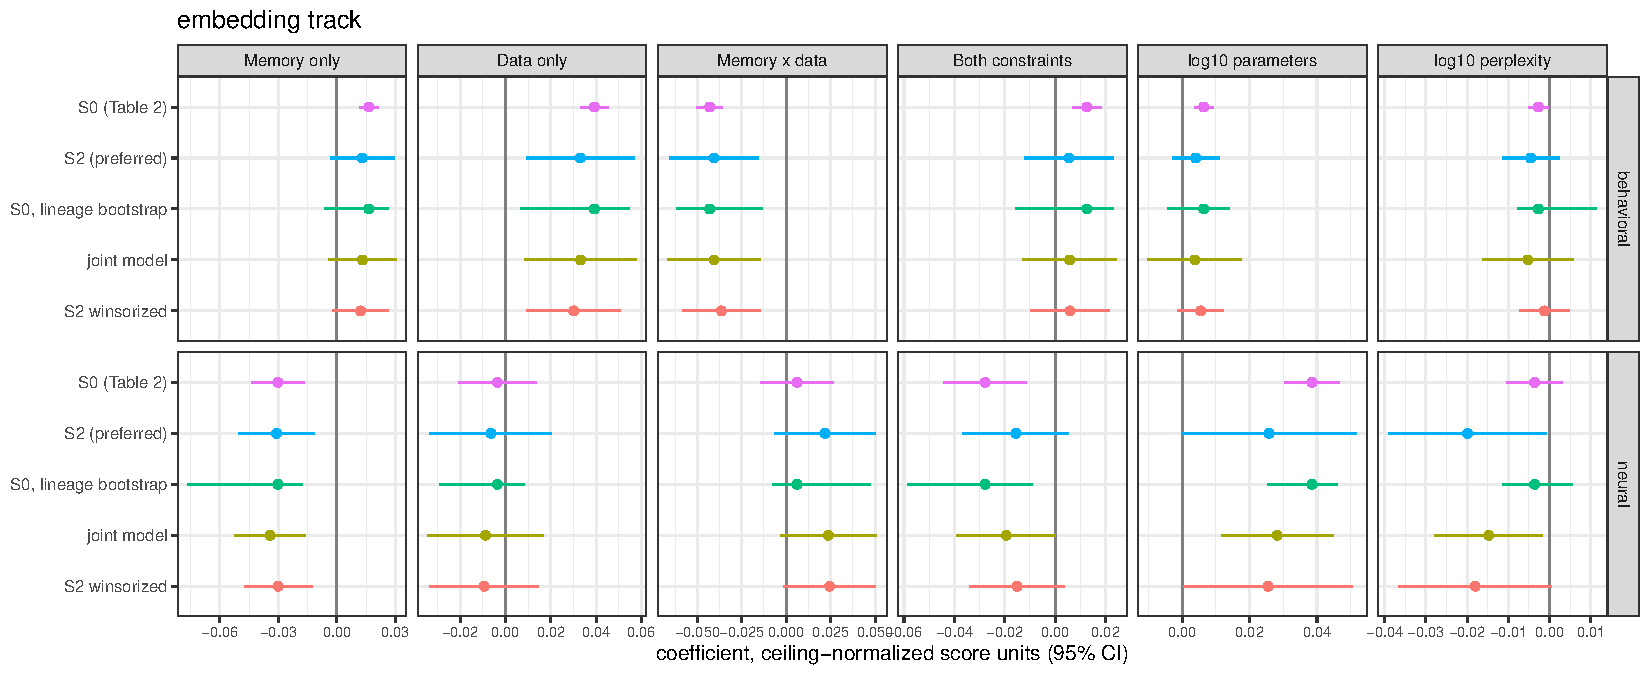
\includegraphics[width=\textwidth]{figures/robust_forest_embedding.pdf}\\[1em]
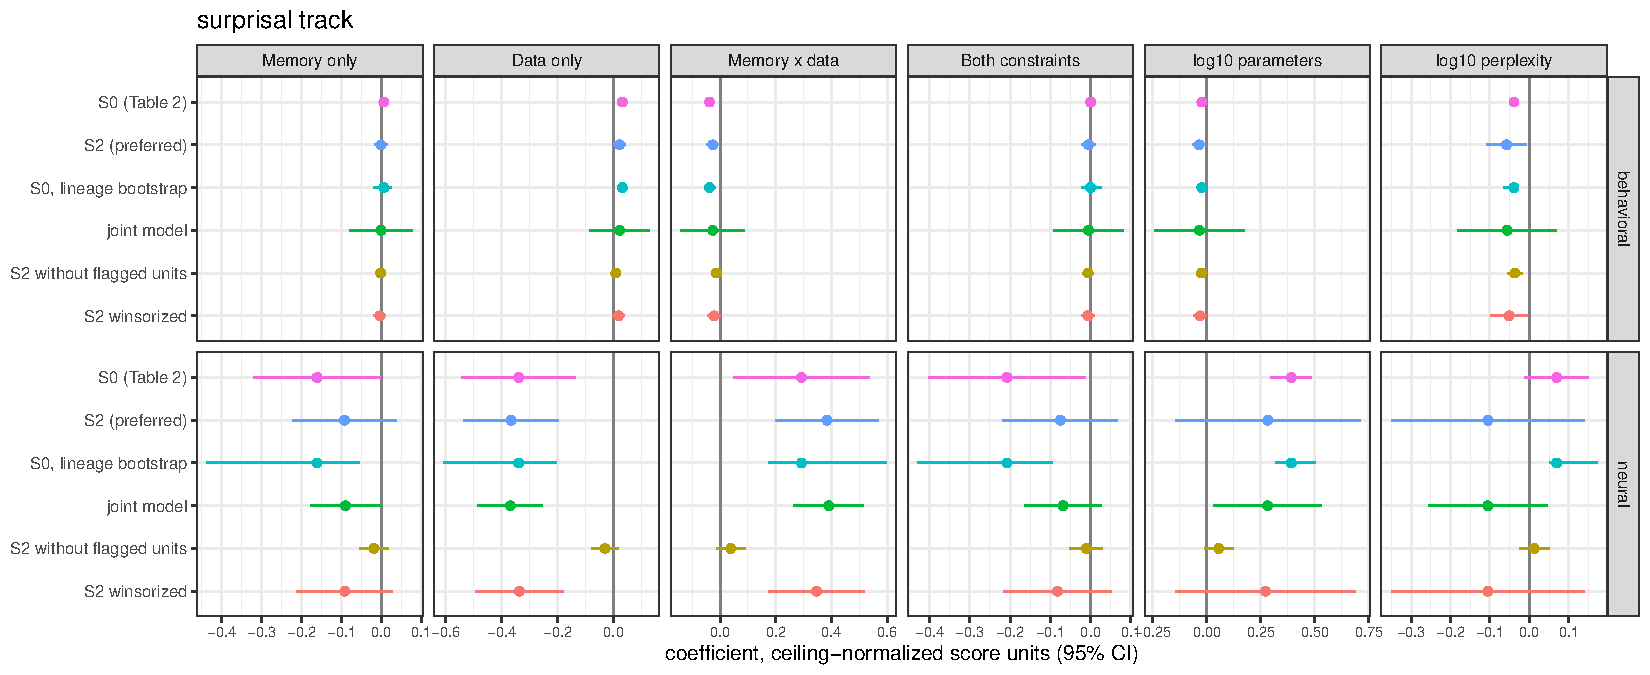
\includegraphics[width=\textwidth]{figures/robust_forest_surprisal.pdf}
\caption{Group associations under the main specifications, embedding track (top) and surprisal track (bottom); points are estimates and bars 95\% intervals in ceiling-normalized score units. S0: dataset-unit random intercept only; S2: preferred specification (Table~\ref{tab:main-regression}); lineage bootstrap: S0 with lineages resampled within constraint groups; joint model: domain-specific effects from the joint behavioral and neural model; the last two rows refit S2 without the units with flagged likelihood references (surprisal only) or with scores winsorized within unit.}
\label{fig:forest}
\end{figure}

\begin{figure}[p]
\centering
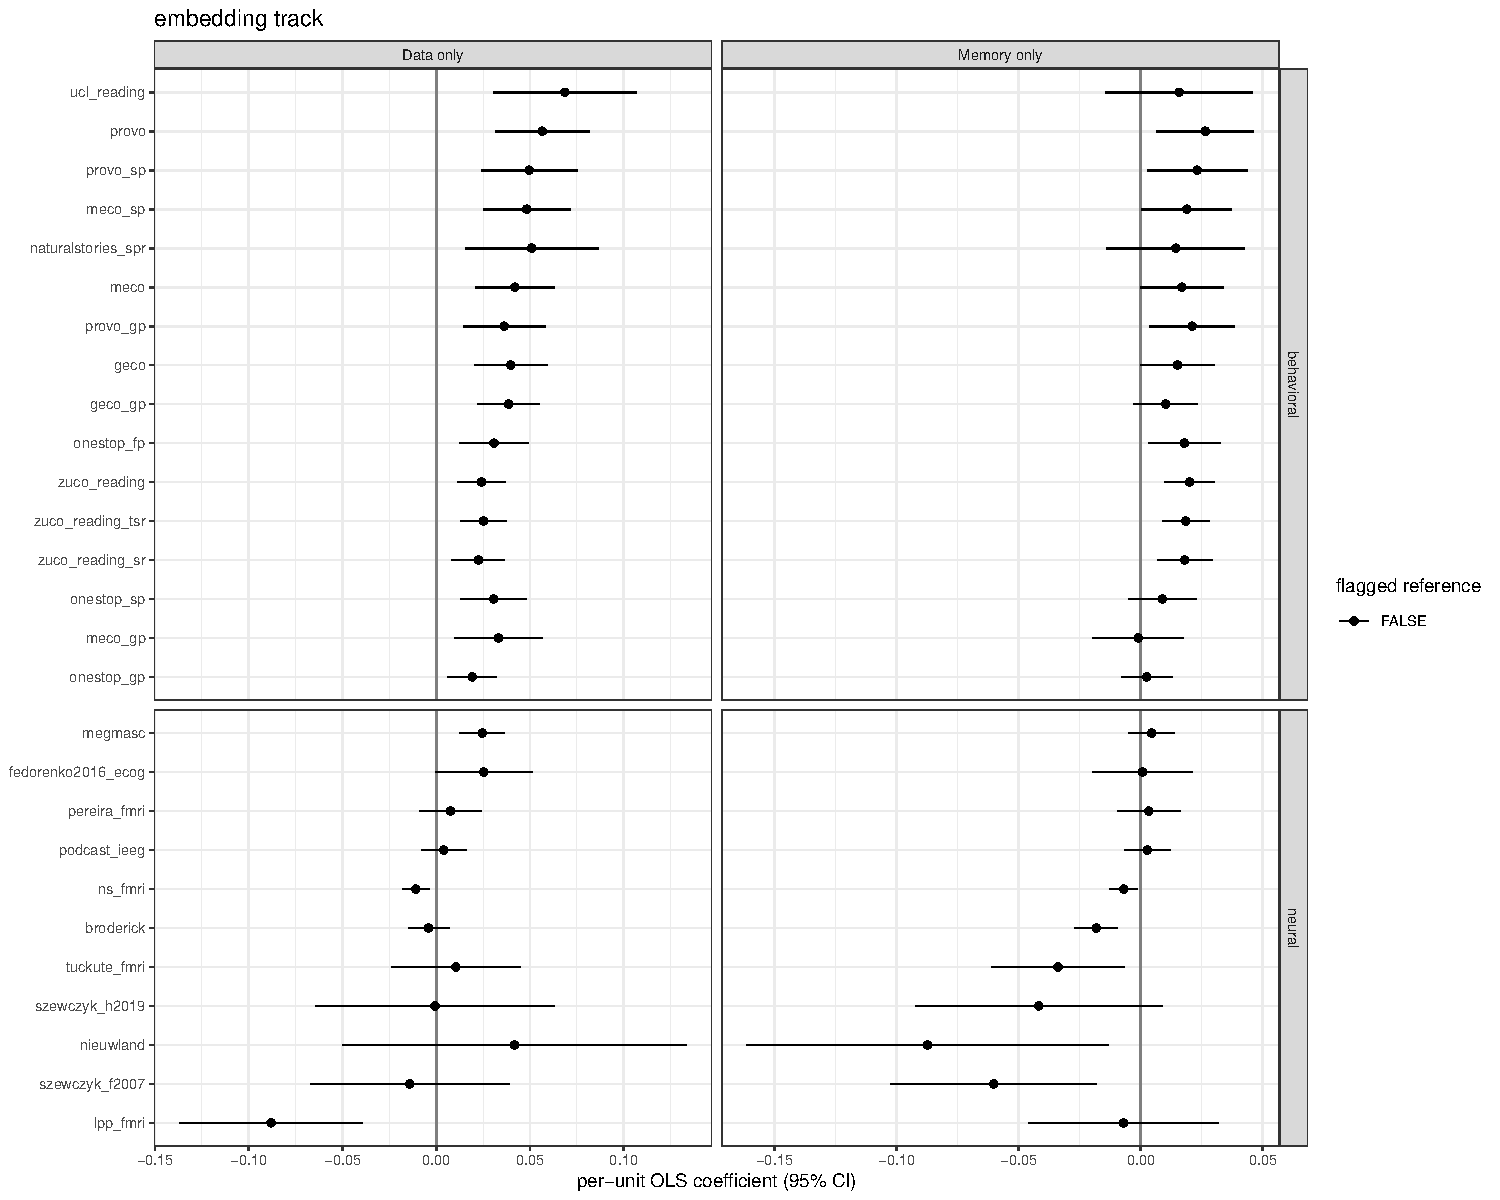
\includegraphics[width=.9\textwidth]{figures/robust_per_unit_embedding.pdf}\\[1em]
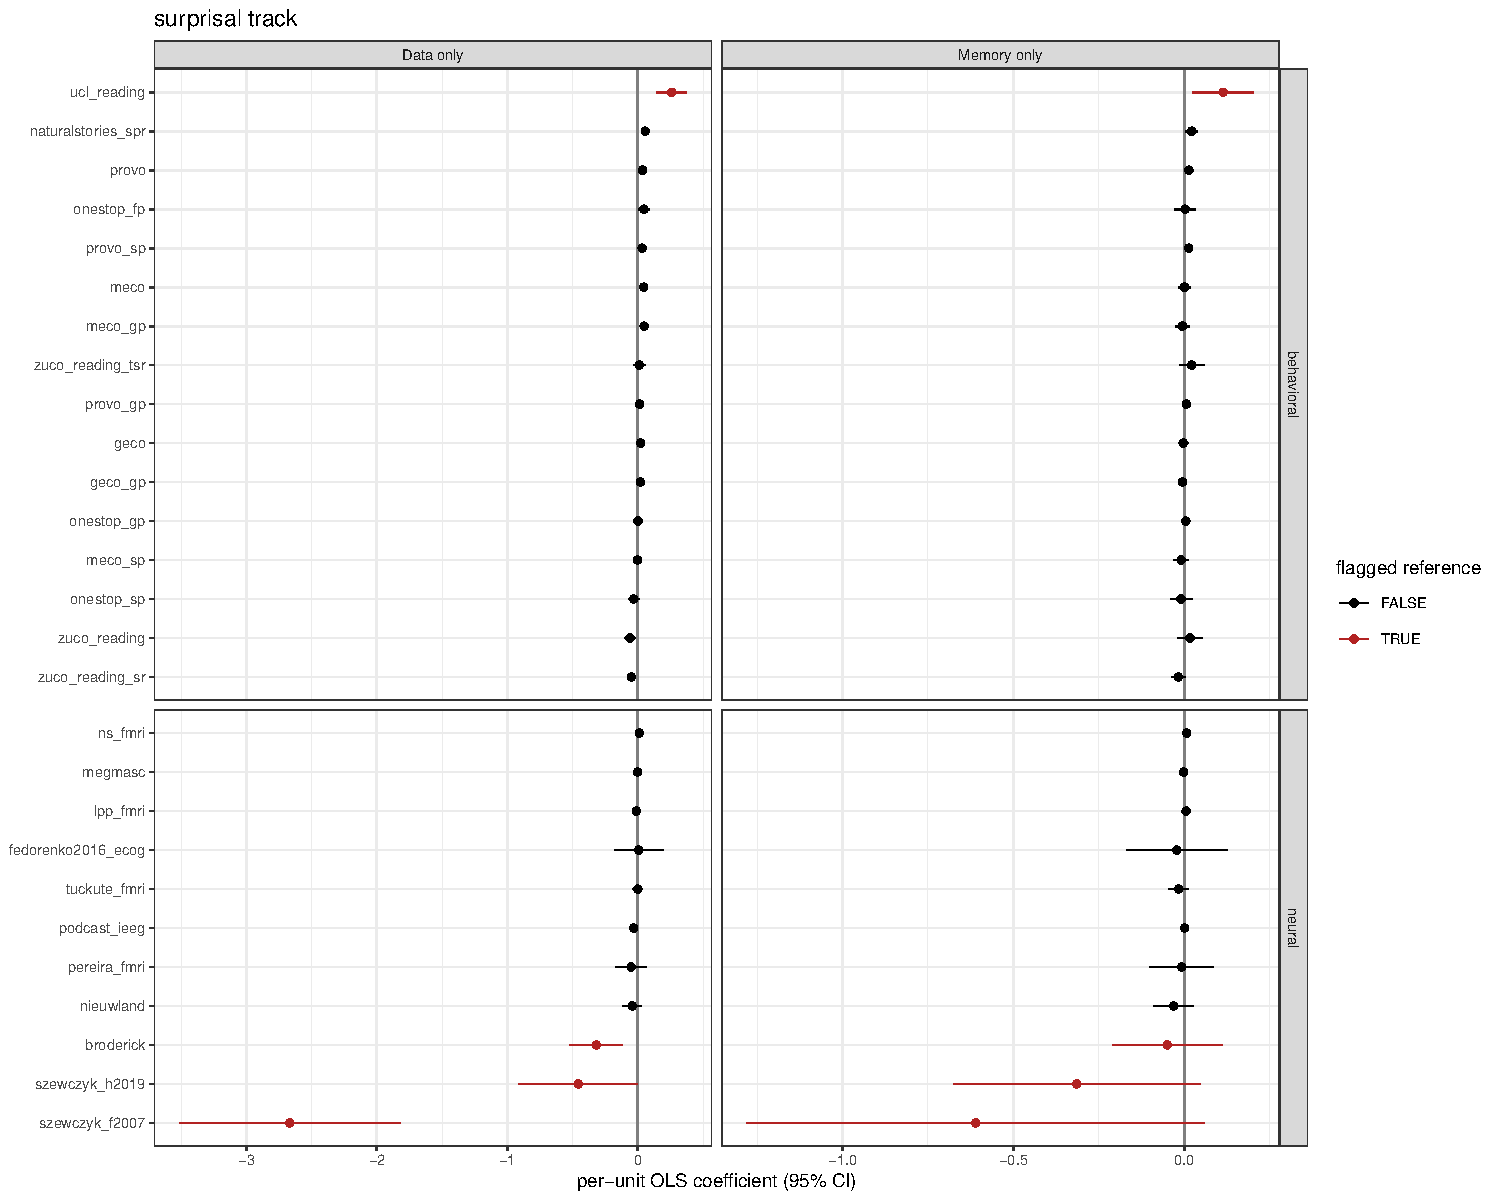
\includegraphics[width=.9\textwidth]{figures/robust_per_unit_surprisal.pdf}
\caption{Memory-only and data-only contrasts estimated separately within each dataset unit (ordinary least squares with size and perplexity, 95\% intervals), embedding track (top) and surprisal track (bottom). Red: units whose likelihood references are flagged in Table~\ref{tab:dll-ceilings}. With about 115 models per unit, single-unit estimates are imprecise; the pooled estimates of Table~\ref{tab:main-regression} borrow strength across units.}
\label{fig:per-unit}
\end{figure}

\section{Design-Based Comparisons: Details}
\label{app:design}

Figure~\ref{fig:dose} shows the scores of the six memory-limited architectures of \citet{bu2026staticlinearattentionconstraints} by training corpus, and Figure~\ref{fig:mechanism} the memory contrasts by mechanism summarized in Table~\ref{tab:design}. Per-architecture fits show the same picture as the pooled within-architecture model. For behavioral embeddings, no architecture predicts reliably better when trained on BabyLM data than on the Pile, and all six predict reliably worse at either 10M or 100M words (by $.005$ to $.032$). For neural embeddings the architectures disagree: the forgetting architecture improves as data decrease ($.035$ at 100M and $.049$ at 10M words), whereas stick-breaking attention is worse at 10M words ($-.059$), so the pooled neural dose-response is not consistent across architectures. These architectures have no softmax-attention counterpart trained on the same three corpora, so the within-architecture comparison isolates the amount of data but cannot test the memory mechanism itself; the Forgetting Transformer pairs provide that test for one mechanism. GPT-BERT models, which combine causal and masked objectives, are evaluated through their causal language-modeling head, so their surprisal is a left-to-right next-token prediction; excluding them does not change the group contrasts (Appendix~\ref{app:robustness}).

\begin{figure}[p]
\centering
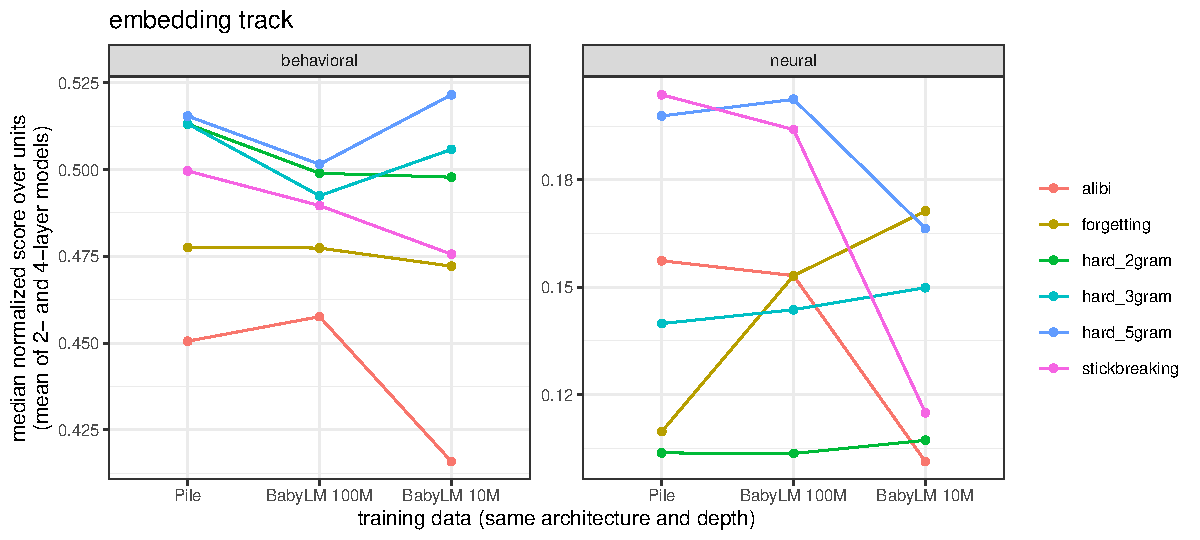
\includegraphics[width=.9\textwidth]{figures/design_dose_embedding.pdf}\\[1em]
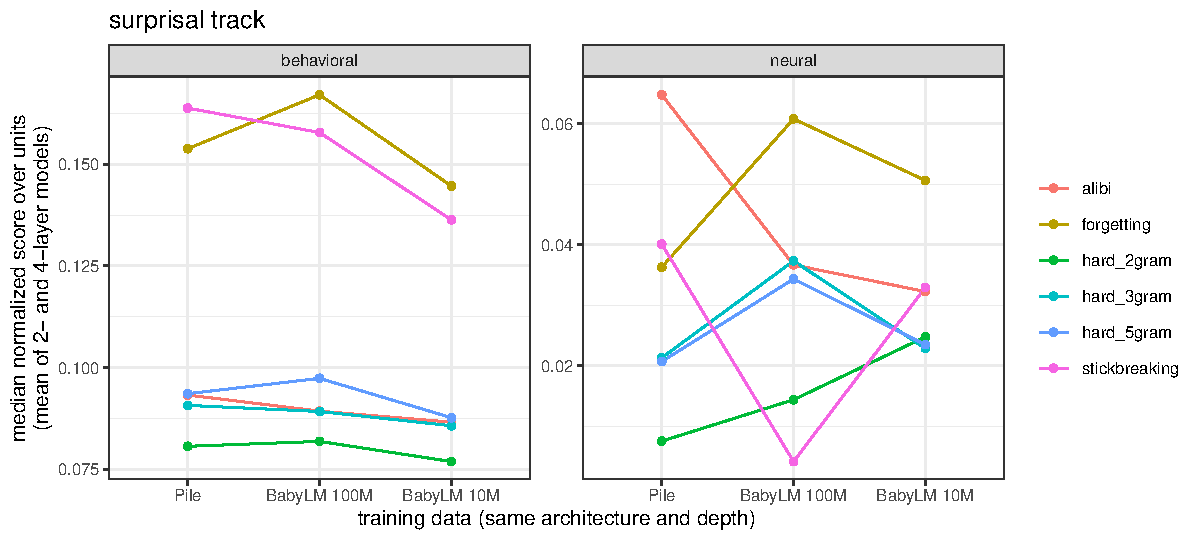
\includegraphics[width=.9\textwidth]{figures/design_dose_surprisal.pdf}
\caption{Within-architecture data comparison, embedding track (top) and surprisal track (bottom). Each line is one memory-limited architecture; points are the median normalized score over dataset units, averaged over the 2- and 4-layer models trained on each corpus.}
\label{fig:dose}
\end{figure}

\begin{figure}[p]
\centering
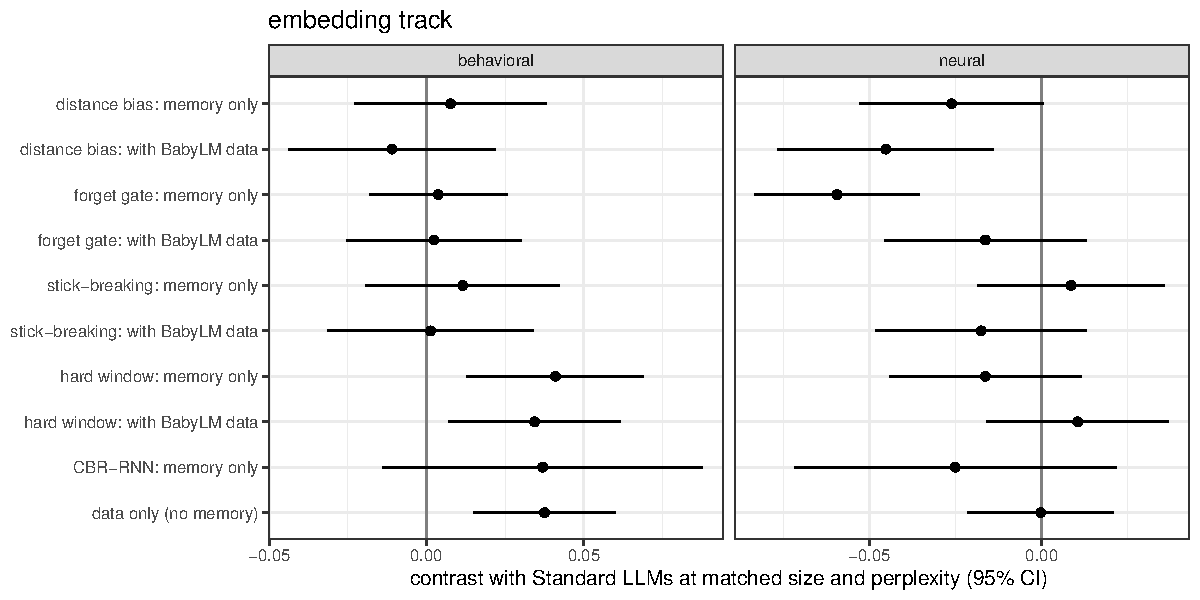
\includegraphics[width=.9\textwidth]{figures/design_mechanism_embedding.pdf}\\[1em]
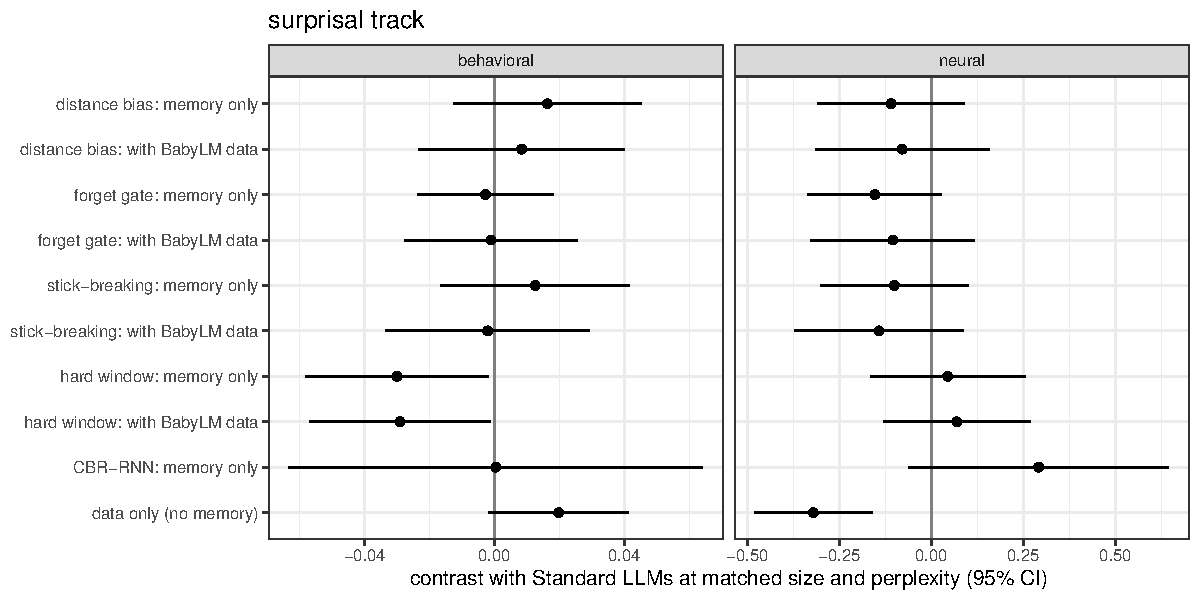
\includegraphics[width=.9\textwidth]{figures/design_mechanism_surprisal.pdf}
\caption{Memory contrasts by mechanism (preferred specification), embedding track (top) and surprisal track (bottom): memory-only contrasts and, for mechanisms also trained on BabyLM data, the combined contrast with Standard LLMs; the last row is the data-only contrast. 95\% intervals.}
\label{fig:mechanism}
\end{figure}

\section{Linear Mixed-Effects Formulas}
\label{app:lme-formulas}

This appendix specifies the linear mixed-effects (LME) models underlying the surprisal track analyses of Section~\ref{sec:design-tracks}, in standard \texttt{lme4} formula notation. All results reported in the paper use the final layer: for each language model and dataset we fit a \emph{baseline} model containing only nuisance covariates, and a \emph{full} model that additionally includes the model's surprisal, with the two compared via the log-likelihood difference described in Appendix~\ref{app:dll-ceiling}. All continuous predictors are z-scored within dataset; \texttt{surprisal\_z} denotes the next-word surprisal of the evaluated model (summed over the word's subword tokens), and \texttt{prev\_surprisal\_z} the same quantity for the preceding word (a spillover control).

\subsection{Self-paced reading and eye-tracking}

Reading times and fixation durations across Natural Stories, UCL Reading, GECO, MECO, Provo, OneStop, and ZuCo Reading are modeled with a common specification, with word length, frequency, and sentence position as nuisance covariates and by-subject random slopes:
\begin{quote}
\texttt{baseline:\ fdur \textasciitilde\ sentpos\_z + wlen\_z + freq\_z +}\\
\texttt{\phantom{baseline:\ fdur \textasciitilde\ }(1 + sentpos\_z + wlen\_z | subject)}\\
\texttt{full:\ fdur \textasciitilde\ sentpos\_z + wlen\_z + freq\_z + surprisal\_z + prev\_surprisal\_z +}\\
\texttt{\phantom{full:\ fdur \textasciitilde\ }(1 + sentpos\_z + wlen\_z + surprisal\_z + prev\_surprisal\_z | subject)}
\end{quote}

\subsection{N400 event-related potentials}

Nieuwland is modeled following the specification of its originating study rather than our shared self-paced-reading/eye-tracking structure, since its multi-site design calls for a different random-effects treatment. Following \citet{nieuwland2018largescale}, laboratory is entered as a fixed rather than random effect, since a random-effect variance is not reliably estimable from only nine sites; there is no electrode term, as N400 amplitude is already averaged across centro-parietal channels in this dataset, nor a frequency covariate, matching the original analysis:
\begin{quote}
\texttt{baseline:\ n400 \textasciitilde\ lab + (1 | subject) + (1 | item)}\\
\texttt{full:\ n400 \textasciitilde\ lab + surprisal\_z + (1 | subject) + (1 | item)}
\end{quote}

Federmeier et al.\ (2007) and Hubbard et al.\ (2019) are fit separately, one model per study, with the specification of the analysis scripts of the Szewczyk and Federmeier collection \citep{szewczyk2022context}. N400 amplitude is pre-averaged over four centro-parietal electrode clusters into one value per trial, so there is no electrode term. The nuisance covariates are the pre-stimulus baseline amplitude (\texttt{bline\_z}), log frequency, word position in the sentence, orthographic neighbourhood (\texttt{old20\_z}) and concreteness, and random slopes are uncorrelated (\texttt{||}); \texttt{item} is the sentence frame:
\begin{quote}
\texttt{baseline:\ n400 \textasciitilde\ bline\_z + freq\_z + pos\_start\_z + old20\_z + concr\_z +}\\
\texttt{\phantom{baseline:\ n400 \textasciitilde\ }(1 + bline\_z + pos\_start\_z || subject) + (1 + bline\_z || item)}\\
\texttt{full:\ n400 \textasciitilde\ bline\_z + freq\_z + pos\_start\_z + old20\_z + concr\_z + surprisal\_z +}\\
\texttt{\phantom{full:\ n400 \textasciitilde\ }(1 + bline\_z + pos\_start\_z || subject) + (1 + bline\_z || item)}
\end{quote}

\subsection{Continuous EEG and MEG}

For Broderick, one model is fit on the data of all subjects pooled, with a random intercept for subject. \texttt{region} denotes four anatomical scalp quadrants (left, right, posterior, occipital), the same for every subject.
\begin{quote}
\texttt{baseline:\ eeg \textasciitilde\ wlen\_z + freq\_z + (1 | subject) + (1 | region)}\\
\texttt{full:\ eeg \textasciitilde\ wlen\_z + freq\_z + surprisal\_z + prev\_surprisal\_z + (1 | subject) + (1 + surprisal\_z | region)}
\end{quote}

For MEG-MASC, the response is the mean amplitude in a 250--450\,ms post-onset window, averaged within six sensor groups (\texttt{region}, the same grouping for every subject); one pooled model is fit over all subjects, with a random intercept for subject. The nuisance covariates are word duration, word length, frequency and the duration of the previous word:
\begin{quote}
\texttt{baseline:\ y \textasciitilde\ worddur\_z + wlen\_z + freq\_z + prev\_worddur\_z + (1 | subject) + (1 | region)}\\
\texttt{full:\ y \textasciitilde\ worddur\_z + wlen\_z + freq\_z + prev\_worddur\_z + surprisal\_z + prev\_surprisal\_z +}\\
\texttt{\phantom{full:\ y \textasciitilde\ }(1 | subject) + (1 + surprisal\_z | region)}
\end{quote}

\subsection{fMRI}

For Natural Stories fMRI, \texttt{story} is a crossed random intercept (there are only eight stories) and the single random slope is on \texttt{subject}; no spillover term is included, since HRF convolution already blends the contributions of adjacent words into a single BOLD sample. Dropping the frequency covariate from both models gives the variant without frequency.
\begin{quote}
\texttt{baseline:\ bold \textasciitilde\ wlen\_z + freq\_z + sentpos\_z + (1 | subject) + (1 | story)}\\
\texttt{full:\ bold \textasciitilde\ wlen\_z + freq\_z + sentpos\_z + surprisal\_z +}\\
\texttt{\phantom{full:\ bold \textasciitilde\ }(1 + surprisal\_z | subject) + (1 | story)}
\end{quote}

For Le Petit Prince, one model is fit on the BOLD signal of all subjects; \texttt{region} denotes one of ten bilateral language-network parcels from the Fedorenko functional atlas, \texttt{section} one of the nine narrative chapters, and \texttt{subject} enters as a random intercept.
\begin{quote}
\texttt{baseline:\ bold \textasciitilde\ wlen\_z + freq\_z + sentpos\_z + (1 | region) + (1 | section) + (1 | subject)}\\
\texttt{full:\ bold \textasciitilde\ wlen\_z + freq\_z + sentpos\_z + surprisal\_z +}\\
\texttt{\phantom{full:\ bold \textasciitilde\ }(1 + surprisal\_z | region) + (1 | section) + (1 | subject)}
\end{quote}

For Tuckute, the response is a single BOLD scalar per (subject, ROI, sentence), so word length and frequency are averaged over the sentence (\texttt{mean\_wlen\_z}, \texttt{mean\_freq\_z}) and surprisal is computed over the whole sentence rather than word-by-word. The model is fit on the naturalistic sentence condition only.
\begin{quote}
\texttt{baseline:\ y \textasciitilde\ mean\_wlen\_z + mean\_freq\_z +}\\
\texttt{\phantom{baseline:\ y \textasciitilde\ }(1 + mean\_wlen\_z + mean\_freq\_z | subject) + (1 | roi) + (1 | sentence\_id)}\\
\texttt{full:\ y \textasciitilde\ mean\_wlen\_z + mean\_freq\_z + surprisal\_z +}\\
\texttt{\phantom{full:\ y \textasciitilde\ }(1 + mean\_wlen\_z + mean\_freq\_z + surprisal\_z | subject) + (1 | roi) +}\\
\texttt{\phantom{full:\ y \textasciitilde\ }(1 + surprisal\_z | sentence\_id)}
\end{quote}

For Pereira, which uses the same per-sentence design as Tuckute but with sentences of variable length, we follow the specification of \citet{linschuler2026surprisal}: sentence length (\texttt{sentlen\_z}) is retained as an additional nuisance covariate alongside mean word length and frequency, and surprisal is again computed over the whole sentence rather than word-by-word. Only two regions of the language-atlas parcellation, the left anterior and left posterior temporal ROIs, carry a reliable sentence-level signal in the split-half $\Delta LL$ ceiling (Appendix~\ref{app:dll-ceiling}); all other ROIs are at noise level. We therefore fit the model separately within each of these two ROIs, so the \texttt{roi} random effect is dropped, normalize each ROI's held-out $\Delta LL$ by its own ceiling, and average the two normalized scores.
\begin{quote}
\texttt{baseline:\ y \textasciitilde\ sentlen\_z + mean\_wlen\_z + mean\_freq\_z +}\\
\texttt{\phantom{baseline:\ y \textasciitilde\ }(1 + sentlen\_z + mean\_wlen\_z + mean\_freq\_z | subject) + (1 | sentence\_id)}\\
\texttt{full:\ y \textasciitilde\ sentlen\_z + mean\_wlen\_z + mean\_freq\_z + surprisal\_z +}\\
\texttt{\phantom{full:\ y \textasciitilde\ }(1 + sentlen\_z + mean\_wlen\_z + mean\_freq\_z + surprisal\_z | subject) +}\\
\texttt{\phantom{full:\ y \textasciitilde\ }(1 + surprisal\_z | sentence\_id)}
\end{quote}

\subsection{Intracranial recordings}

For Fedorenko2016, electrodes are patient-specific, so \texttt{electrode} is nested within \texttt{subject} rather than treated as a crossed effect. Podcast is instead fit per region on region-averaged electrodes, so no electrode term is needed: for each language region (anterior temporal, inferior frontal, posterior temporal; left-hemisphere electrodes assigned to the Fedorenko language parcels, with the orbital part of the inferior frontal gyrus merged into the inferior frontal region and the middle frontal gyrus dropped because it has fewer than four subjects), the high-gamma response is averaged over the region's electrodes within each subject and word, and the model is fit separately at each lag of the 0--600\,ms post-onset window (19 lags on the 31.25\,ms grid), at the final layer; no spillover term is included. Responses are standardized with statistics computed on the training chunks only (per electrode, then per subject and region after averaging) and applied unchanged to the held-out chunks, so no information from the held-out data enters the scaling. The headline score is the mean over lags of the held-out $\Delta LL$ per observation of each region, divided by that region's own noise ceiling and then averaged across regions weighted by their number of held-out observations.
\begin{quote}
\texttt{baseline:\ y \textasciitilde\ wlen\_z + freq\_z + (1 | subject)}\\
\texttt{full:\ y \textasciitilde\ wlen\_z + freq\_z + surprisal\_z + (1 | subject)}
\end{quote}

For Fedorenko2016, spillover is included, along with a richer by-subject random-slope structure:
\begin{quote}
\texttt{baseline:\ y \textasciitilde\ wlen\_z + freq\_z + (1 + wlen\_z + freq\_z | subject) +}\\
\texttt{\phantom{baseline:\ y \textasciitilde\ }(1 | subject:electrode)}\\
\texttt{full:\ y \textasciitilde\ wlen\_z + freq\_z + surprisal\_z + prev\_surprisal\_z +}\\
\texttt{\phantom{full:\ y \textasciitilde\ }(1 + wlen\_z + freq\_z + surprisal\_z + prev\_surprisal\_z | subject) +}\\
\texttt{\phantom{full:\ y \textasciitilde\ }(1 + surprisal\_z + prev\_surprisal\_z | subject:electrode)}
\end{quote}


\section{Representational Evaluation}
\label{app:rsa}

The ridge encoders of the embedding track have a number of free parameters that grows with the hidden size $d$ of the model, so a score that increases with model size may reflect the capacity of the regression rather than a better representation. Representational similarity analysis (RSA; \citealp{kriegeskorte2008rsa}) removes this dependence: whatever $d$ is, a model yields one stimulus-by-stimulus dissimilarity matrix (RDM), and the downstream score involves at most a single model coefficient, with no per-feature weights and no tuned hyperparameter. We run it for both tracks, on the same models and stimuli as the main benchmark and with the final layer of each model. The subsections below describe the dissimilarity matrices, the unfitted RSA score, the confound-controlled RDM regression with its cross-validation, the noise ceilings, and the aggregation.

\subsection{Dissimilarity matrices}
\label{app:rsa-rdms}

For each stimulus $i$, let $h_i$ denote its final-layer embedding and $s_i$ its surprisal. Embedding features are standardized across the scored stimuli, $\widetilde h_{ik}=(h_{ik}-\mu_k)/\sigma_k$, with constant features set to zero. This preprocessing addresses unequal feature scales \citep{timkey2021allbark}; it is distinct from standardizing outcome scores across models. Because the statistics include all scored stimuli, it is a transductive transformation, although it uses no response values. Raw last-layer states of Transformers contain a handful of high-magnitude dimensions that dominate cosine and correlation distances \citep{timkey2021allbark}, which is why every feature is standardized before distances are computed. Surprisal $s_i$ is the surprisal of the (critical) word, or the summed surprisal of the sentence for sentence-level datasets, exactly as used by the mixed-effects analyses. Model distances are
\[
D^E_{ij}=1-\operatorname{corr}(\widetilde h_i,\widetilde h_j),\qquad D^S_{ij}=|s_i-s_j|.
\]
Behavioral distances are absolute differences in item-mean reading responses. Scalar N400 responses are treated analogously; multivariate neural response patterns use correlation distance. Stimulus alignment and response aggregation are dataset-specific. The current RSA Pareto analysis uses language-region units for Pereira and Tuckute, language parcels for Podcast, regional responses for Broderick and MEG-MASC, and the three N400 datasets.

All stimulus pairs are used where feasible; GECO and OneStop use a fixed random sample of 30 million pairs, the same for every model. Model, response, nuisance, and ceiling quantities use corresponding pairs within each analysis. The per-dataset correlations of Table~\ref{tab:rsa-summary} use each dataset's full response RDM rather than the regional units of the Pareto composites, so their values are not directly comparable with those composites.

\subsection{Unfitted Pearson RSA}
\label{app:rsa-scores}

Let $v(D)$ denote the retained upper-triangle entries. Unfitted RSA is
\[
R=\operatorname{corr}\bigl(v(D^{\mathrm{model}}),v(D^{\mathrm{response}})\bigr).
\]
It learns no weights mapping model features to responses and does not remove lexical confounds. The neural RSA Pareto score divides each response unit's RSA by its own positive RSA ceiling, summarizes these ratios by the median within a dataset, and takes the median across the eight neural datasets. Behavioral composites take the median across the 16 measure-specific ratios. All 118 plotted models have complete coverage at these dataset/measure levels. The RSA ceiling uses the square root of Spearman--Brown-corrected split-half RDM reliability.

\subsection{Confound-controlled RDM regression}
\label{app:rsa-cv}

For each retained pair, the nuisance model predicts response distance from an intercept and absolute differences in word length and frequency. The full model adds one model-distance predictor:
\begin{align*}
D^{\mathrm{response}}_{ij}&=a+b_LD^{\mathrm{length}}_{ij}+b_FD^{\mathrm{frequency}}_{ij}+e_{ij},\\
D^{\mathrm{response}}_{ij}&=a+b_LD^{\mathrm{length}}_{ij}+b_FD^{\mathrm{frequency}}_{ij}+b_MD^{\mathrm{model}}_{ij}+e_{ij}.
\end{align*}
For Federmeier et al.\ (2007) and Hubbard et al.\ (2019), the nuisance model additionally includes absolute differences in word position, orthographic neighborhood (OLD20) and concreteness, to match the covariates of their published mixed-effects formulas; for sentence datasets, the lexical distances are computed from sentence length, mean word length and mean word frequency. Random-effect structures have no counterpart on an item-averaged target and are not reproduced. All distance entries are z-scored before fitting. The models are fit by ordinary least squares, and Gaussian test log likelihood uses the variance estimated from training residuals. The score is the full-minus-baseline test log likelihood per pair. There is one model-distance coefficient regardless of embedding width; no feature reweighting is fitted.

Cross-validation partitions stimuli. For a held-out fold, training pairs have both stimuli outside the fold and test pairs have both inside it; pairs crossing the boundary are omitted. This prevents training and test pairs from sharing stimuli in a split \citep{schutt2023statistical}. Following \citet{schutt2023statistical}, the number of folds depends on the number of stimuli $n$: $K=2$ for $n<12$, 3 for $12\le n<24$, 4 for $24\le n<40$, and 5 for $n\ge 40$. Test log likelihoods are summed over folds, and the procedure is repeated with new random partitions (10 by default), the reported score being the mean over repeats. Partitions are fixed per dataset and unit, so all models and both tracks are scored on identical train and test pairs, and base and full models are always compared on the same test pairs. Pairs sharing a stimulus remain correlated within the training and test sets, which violates the independence assumption of the Gaussian likelihood and inflates absolute values by roughly the same amount for all models. The pair likelihood is therefore used to rank models, not as a source of independent-pair significance tests, and its absolute scale is not interpreted. Negative scores indicate worse held-out fit than the nuisance baseline.

Figure~\ref{fig:rdm-pareto} uses dataset- and measure-level RDM-regression scores, divided by the matching split-half likelihood references and then aggregated by medians. This differs from the unit-wise Pearson RSA normalization described above. In both cases, only usable positive references enter the composite; negative model scores and ratios above one are retained. Normalization does not make the direct-prediction, Pearson RSA, and RDM-likelihood scales interchangeable.

\subsection{Noise ceilings for representational scores}
\label{app:rsa-ceilings}

Both representational scores are expressed relative to the reliability of the human data, computed in the same RDM space, with the same item folds, nuisance RDMs and pair likelihood as the models. Participants are randomly split into two equal halves $A$ and $B$ (15 splits); items must be observed in both halves. For neural datasets the split is over subjects and is carried out separately for each response unit (ROI, channel, region, or region $\times$ lag), so each unit has its own ceiling.

\paragraph{RSA-correlation ceiling.} The split-half reliability $r_{\mathrm{half}}$ is the Pearson correlation between the entries of the two half-sample response RDMs, averaged over splits and extrapolated by the Spearman--Brown formula; the ceiling for a correlation is $\sqrt{r_{\mathrm{SB}}}$, as in Appendix~\ref{app:corr-ceiling}. Units whose $r_{\mathrm{half}}$ is not positive have no defined ceiling and are excluded.

\paragraph{Split-half $\Delta\ell$ reference.} Half $A$'s item-mean RDM is used as the predictor of half $B$'s item-mean RDM in the full model above, in place of a model RDM, and compared with the same nuisance-only baseline on the same test pairs; the roles of $A$ and $B$ are then swapped, the two totals are summed and divided by the total number of test pairs, and the reference is the mean over splits. The predictor is built from only half of the participants, so the reference is conservative and no Spearman--Brown correction is available on the likelihood scale; ratios above 1 can occur.

Table~\ref{tab:rsa-ceilings} reports the RSA-correlation references with the number of usable units, and Table~\ref{tab:rdm-dll-ceilings} the RDM-regression references used in Figure~\ref{fig:rdm-pareto}.

{\small\setlength{\tabcolsep}{4pt}
\begin{longtable}{@{}lrrrr@{}}
\caption{RSA-correlation references and maximum final-layer normalized scores. For neural datasets, Reference is the median of the unit-level ceilings, reported for context; normalization is performed within units before taking the median and is not division by this displayed summary. Units counts usable positive-ceiling response units. For behavioral measures there is one ceiling per measure. Maximum columns are maxima across models of the dataset/measure score.}\label{tab:rsa-ceilings} \\
\toprule
Dataset / measure & Reference & Units & Max. emb. & Max. sur. \\
\midrule
\endfirsthead
\multicolumn{5}{c}{\tablename\ \thetable{} -- continued} \\
\toprule
Dataset / measure & Reference & Units & Max. emb. & Max. sur. \\
\midrule
\endhead
\midrule\multicolumn{5}{r}{Continued on next page} \\
\endfoot
\bottomrule
\endlastfoot
Pereira fMRI & 0.260 & 20 & 0.152 & 0.058 \\
Tuckute fMRI & 0.288 & 13 & 0.072 & 0.176 \\
Podcast ECoG & 0.224 & 122 & 0.050 & 0.059 \\
Broderick EEG & 0.105 & 4 & 0.020 & 0.111 \\
MEG-MASC & 0.154 & 6 & 0.018 & 0.047 \\
Nieuwland N400 & 0.787 & 1 & 0.118 & 0.185 \\
Federmeier 2007 N400 & 0.363 & 1 & 0.171 & 0.649 \\
Hubbard 2019 N400 & 0.517 & 1 & 0.204 & 0.554 \\
Provo / FP & 0.863 & 1 & 0.130 & 0.458 \\
Provo / GP & 0.735 & 1 & 0.049 & 0.252 \\
Provo / SP & 0.884 & 1 & 0.129 & 0.460 \\
MECO / FP & 0.842 & 1 & 0.139 & 0.425 \\
MECO / GP & 0.487 & 1 & 0.043 & 0.125 \\
MECO / SP & 0.899 & 1 & 0.147 & 0.456 \\
UCL / SPR & 0.505 & 1 & 0.017 & 0.177 \\
ZuCo / NR & 0.766 & 1 & 0.125 & 0.555 \\
ZuCo / SR & 0.799 & 1 & 0.104 & 0.501 \\
ZuCo / TSR & 0.555 & 1 & 0.099 & 0.361 \\
Natural Stories / SPR & 0.873 & 1 & 0.033 & 0.254 \\
GECO / GP & 0.296 & 1 & 0.031 & 0.117 \\
GECO / FP & 0.420 & 1 & 0.067 & 0.272 \\
OneStop / GP & 0.526 & 1 & 0.022 & 0.136 \\
OneStop / SP & 0.666 & 1 & 0.073 & 0.415 \\
OneStop / FP & 0.566 & 1 & 0.054 & 0.419 \\
\end{longtable}
}


{\small\setlength{\tabcolsep}{4pt}
\begin{longtable}{@{}lrc@{}}
\caption{Dataset/measure-level split-half likelihood references for the RDM-regression fronts in Figure~\ref{fig:rdm-pareto}, in $\Delta\ell$ per pair. They differ from the unit-wise normalization of the RSA correlations. All listed references are positive.}\label{tab:rdm-dll-ceilings} \\
\toprule
Dataset / measure & Reference & Included \\
\midrule
\endfirsthead
\multicolumn{3}{c}{\tablename\ \thetable{} -- continued} \\
\toprule
Dataset / measure & Reference & Included \\
\midrule
\endhead
\midrule\multicolumn{3}{r}{Continued on next page} \\
\endfoot
\bottomrule
\endlastfoot
Pereira fMRI & $2.98\times10^{-4}$ & Yes \\
Tuckute fMRI & $3.53\times10^{-4}$ & Yes \\
Broderick EEG & $3.28\times10^{-5}$ & Yes \\
MEG-MASC & $8.08\times10^{-5}$ & Yes \\
Podcast ECoG & $3.46\times10^{-4}$ & Yes \\
Nieuwland N400 & $1.11\times10^{-1}$ & Yes \\
Federmeier 2007 N400 & $1.95\times10^{-3}$ & Yes \\
Hubbard 2019 N400 & $9.01\times10^{-3}$ & Yes \\
Provo / FP & $1.69\times10^{-1}$ & Yes \\
Provo / GP & $7.36\times10^{-2}$ & Yes \\
Provo / SP & $2.13\times10^{-1}$ & Yes \\
MECO / FP & $1.42\times10^{-1}$ & Yes \\
MECO / GP & $7.13\times10^{-3}$ & Yes \\
MECO / SP & $2.67\times10^{-1}$ & Yes \\
GECO / FP & $3.64\times10^{-3}$ & Yes \\
GECO / GP & $8.60\times10^{-4}$ & Yes \\
OneStop / FP & $1.25\times10^{-2}$ & Yes \\
OneStop / GP & $1.22\times10^{-2}$ & Yes \\
OneStop / SP & $3.09\times10^{-2}$ & Yes \\
Natural Stories / SPR & $2.33\times10^{-1}$ & Yes \\
UCL / SPR & $9.74\times10^{-3}$ & Yes \\
ZuCo / NR & $7.40\times10^{-2}$ & Yes \\
ZuCo / SR & $9.17\times10^{-2}$ & Yes \\
ZuCo / TSR & $1.34\times10^{-2}$ & Yes \\
\end{longtable}
}


\subsection{Scaling and agreement with direct prediction}
\label{app:rsa-panels}

Table~\ref{tab:rsa-summary} reports descriptive correlations across the 118 models, computed from the per-model RSA and direct-prediction scores with the current group assignments. The size columns correlate RSA with $\log_{10}$ parameter count, pooled over all models and within constraint groups (the partial correlation controlling for group membership). The agreement columns correlate embedding RSA with direct embedding Pearson scores, and surprisal RSA with direct surprisal $\Delta\ell$ scores. These correlations are not adjusted for model family and do not test a difference between behavioral and neural correlations.

\begin{table}[p]
\centering\small
\caption{Descriptive Pearson correlations across 118 models: RSA with $\log_{10}$ parameter count (size), the same correlation within constraint groups (partial correlation controlling for group membership, so that it does not merely reflect that the smallest models are the constrained ones), and RSA with the corresponding direct-prediction score (agreement: embedding RSA with encoding $r$, surprisal RSA with surprisal $\Delta\ell$). Emb.\ denotes embeddings; Sur.\ denotes surprisal. No model-family adjustment or significance test is applied.}
\label{tab:rsa-summary}
\begin{tabular}{lrrrrrr}
\toprule
& \multicolumn{2}{c}{Size} & \multicolumn{2}{c}{Size within group} & \multicolumn{2}{c}{Agreement}\\
\cmidrule(lr){2-3}\cmidrule(lr){4-5}\cmidrule(lr){6-7}
Dataset / measure & Emb. & Sur. & Emb. & Sur. & Emb. & Sur.\\
\midrule
Pereira / fMRI & 0.698 & 0.177 & 0.460 & 0.056 & 0.420 & 0.019 \\
Tuckute B / fMRI & 0.437 & 0.603 & 0.165 & 0.302 & 0.820 & 0.564 \\
Broderick / EEG & 0.606 & -0.070 & 0.371 & 0.267 & 0.733 & -0.119 \\
MEG-MASC / MEG & -0.558 & 0.550 & -0.444 & 0.305 & 0.275 & 0.138 \\
Nieuwland / N400 & 0.717 & 0.729 & 0.526 & 0.629 & 0.532 & 0.749 \\
Federmeier et al. (2007) / N400 & 0.884 & 0.795 & 0.762 & 0.558 & 0.929 & 0.751 \\
Hubbard et al. (2019) / N400 & 0.729 & 0.739 & 0.545 & 0.569 & 0.823 & 0.517 \\
Podcast / ECoG & 0.475 & 0.131 & 0.365 & -0.127 & 0.769 & 0.442 \\
\midrule
Provo / FP & -0.494 & -0.397 & -0.183 & -0.311 & 0.678 & 0.354 \\
Provo / GP & -0.259 & -0.527 & -0.020 & -0.294 & 0.663 & 0.017 \\
Provo / SP & -0.498 & -0.037 & -0.192 & -0.113 & 0.649 & 0.243 \\
MECO English / FP & -0.597 & -0.339 & -0.256 & -0.214 & 0.154 & 0.584 \\
MECO English / GP & -0.394 & -0.381 & -0.044 & -0.266 & 0.087 & -0.194 \\
MECO English / SP & -0.582 & -0.058 & -0.228 & -0.067 & 0.117 & 0.227 \\
GECO / FP & -0.366 & -0.397 & -0.082 & -0.240 & 0.023 & -0.272 \\
GECO / GP & -0.133 & -0.669 & 0.018 & -0.438 & -0.359 & -0.304 \\
OneStop / FP & -0.519 & 0.186 & -0.234 & 0.135 & -0.342 & 0.284 \\
OneStop / GP & 0.153 & -0.813 & 0.107 & -0.654 & 0.031 & -0.206 \\
OneStop / SP & -0.457 & 0.562 & -0.142 & 0.336 & -0.412 & 0.751 \\
Natural Stories / SPR & 0.101 & 0.192 & 0.121 & 0.202 & 0.388 & 0.132 \\
UCL Reading / SPR & -0.043 & 0.507 & 0.088 & 0.418 & 0.577 & 0.715 \\
ZuCo / NR & -0.623 & 0.043 & -0.337 & 0.024 & -0.325 & 0.248 \\
ZuCo / SR & -0.245 & 0.458 & -0.003 & 0.335 & -0.219 & 0.399 \\
ZuCo / TSR & -0.643 & 0.545 & -0.360 & 0.378 & -0.007 & 0.694 \\
\bottomrule
\end{tabular}
\end{table}


